\makeatletter
  \graphicspath{ {\import@path} }
\makeatother

\begin{frame}[fragile]{Introduction}
  \begin{columns}

    \begin{column}{0.5\textwidth}
      \begin{itemize}
        \item Zero-Permutation Jet-Parton Assignment using a Self-Attention Network
        \item \href{https://doi.org/10.48550/arXiv.2012.03542}{arXiv:2012.03542} (\href{https://inspirehep.net/literature/1835305}{12 citations})
        \item \href{https://pos.sissa.it/390/348}{Presented in the oral session at International Conference on High Energy Physics 2020}
      \end{itemize}
    \end{column}

    \begin{column}{0.5\textwidth}
      \begin{figure}[htpb]
        \centering
        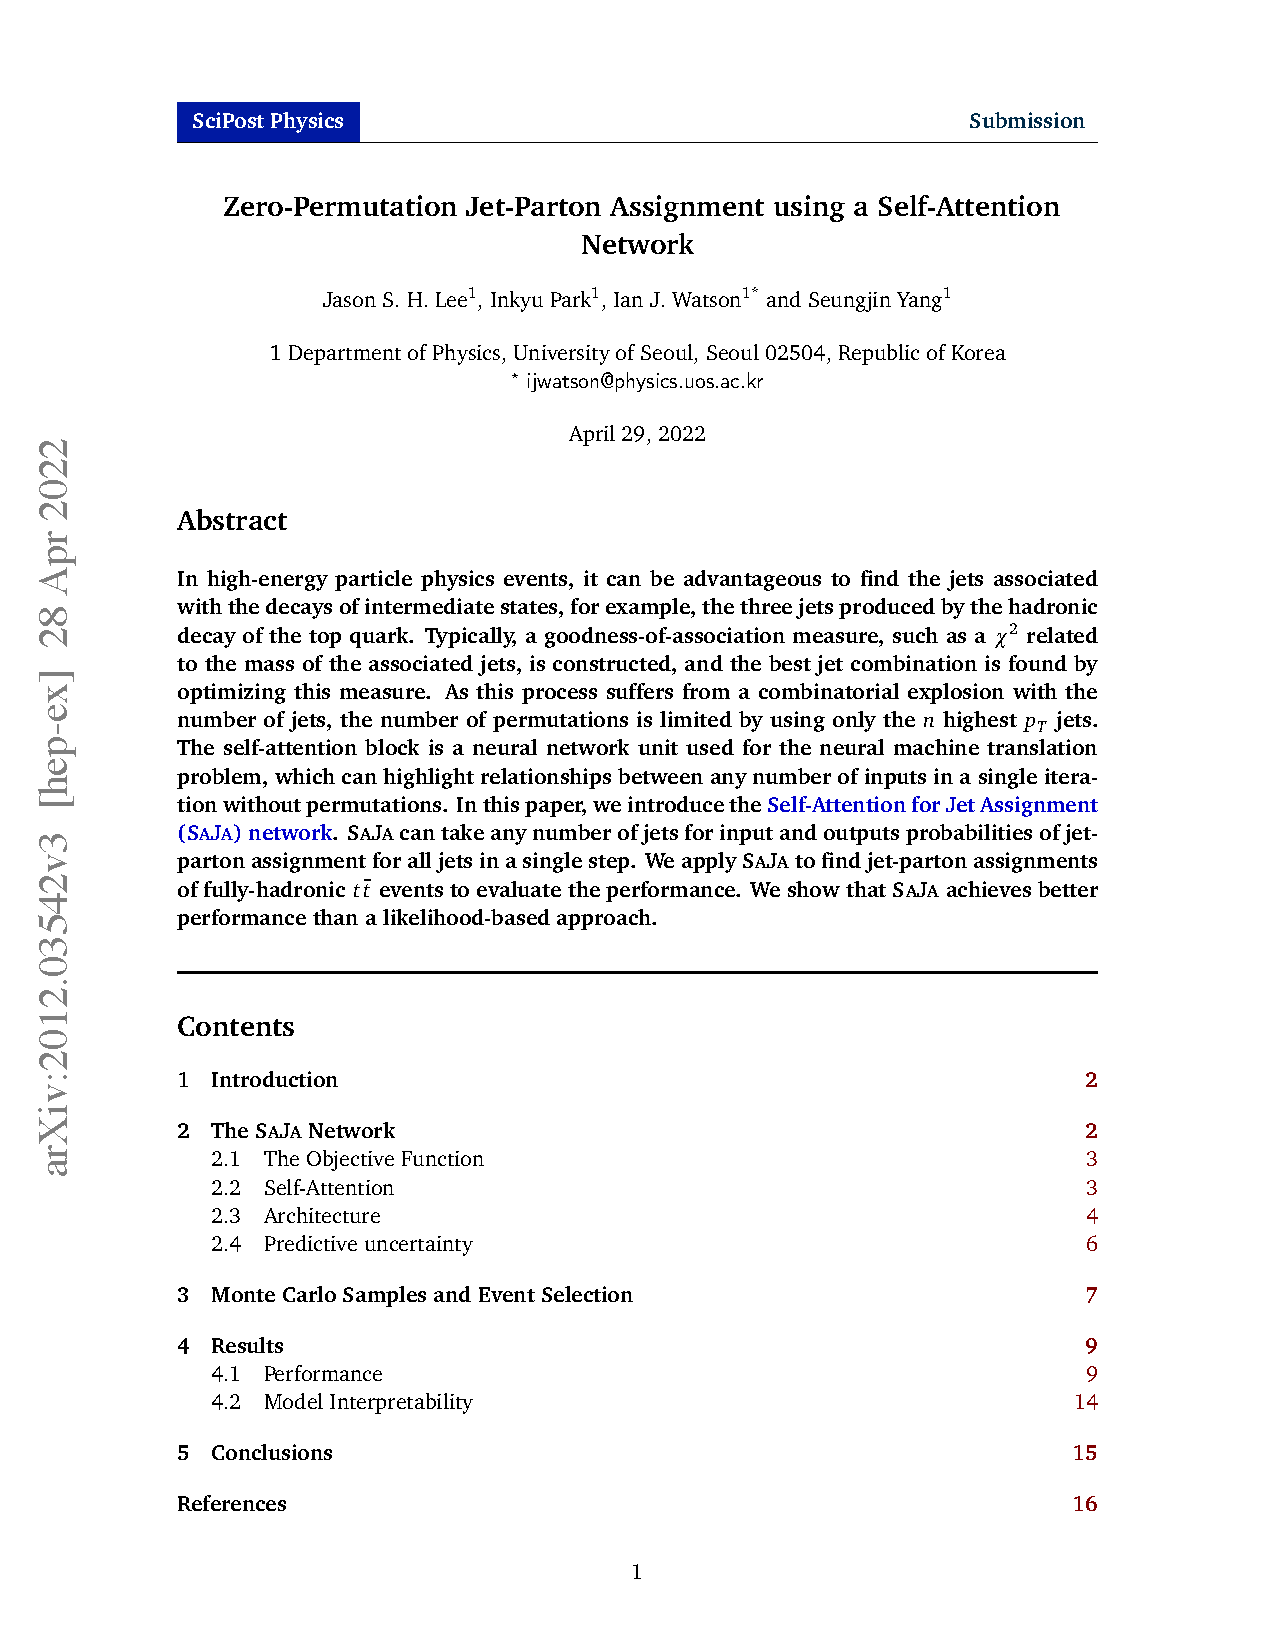
\includegraphics[height=0.48\textheight]{fig/publication/2012.03542.pdf}
      \end{figure}
      
    \end{column}

  \end{columns}
\end{frame}

\begin{frame}[fragile]{Introduction}
\begin{columns}
    \column{0.65\textwidth}
    \begin{itemize}
      \item[$\bullet$] The reconstruction of events with intermediate states 
                       decaying to jets requires a technique to assign jets to partons.
      \item[$\bullet$] The number of jets can be greater than the number of 
                       partons because of additional QCD radiation. It makes the assignment harder.
      \item[$\bullet$] We introduce {\bfseries the self-attention for jet
                       assignment (SAJA) network without requiring jet permutations}.
                       We apply SAJA, to find jet-parton assignments of
                       fully-hadronic \ttbar events to test the performance.
    \end{itemize}
    \column{0.35\textwidth}
    \begin{figure}[htpb]
      \centering
      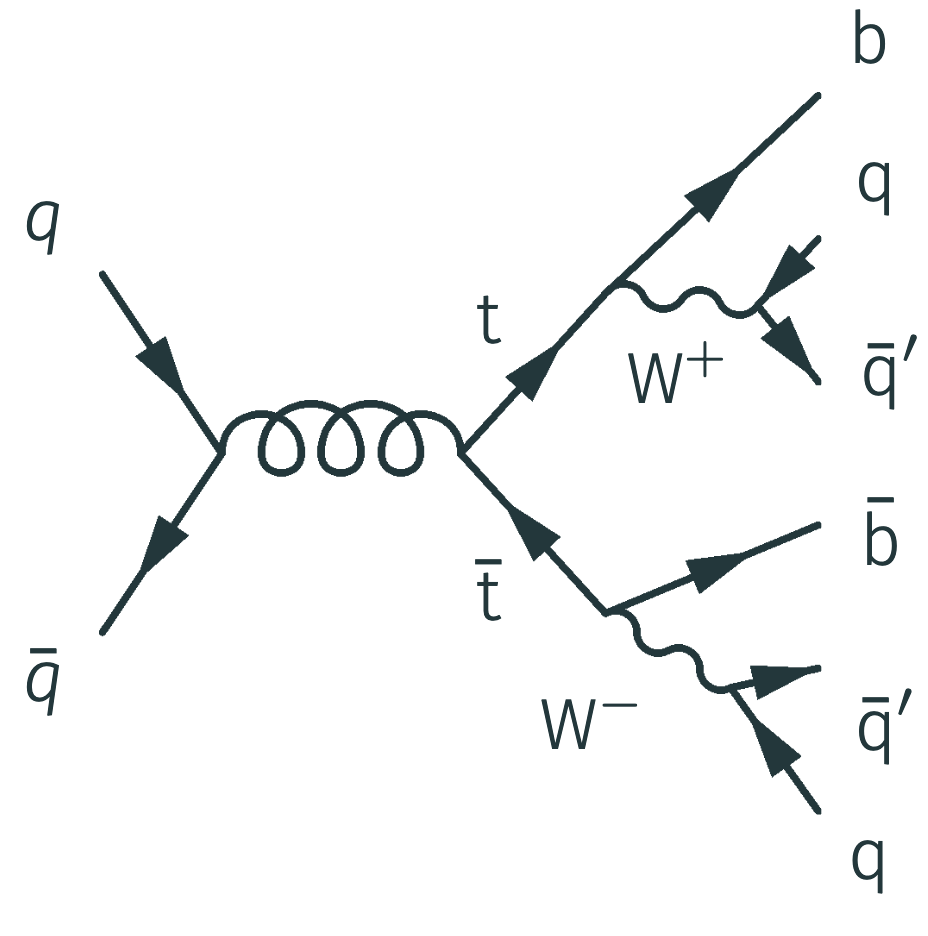
\includegraphics[width=0.8\textwidth]{fig/ttbar.png}
    \end{figure}
\end{columns}
\end{frame}

%%%%%%%%%%%%%%%%%%%%%%%%%%%%%%%%%%%%%%%%%%%%%%%%%%%%%%%%%%%%%%%%%%%%%%%%%%%%%%%
\begin{frame}[fragile]{Preceding Research}
  \begin{block}{$\blacksquare$ $\chi^{2}$ method {\scriptsize \href{https://link.springer.com/article/10.1140\%2Fepjc\%2Fs10052-019-6788-2}{[CMS, Eur. Phys. J. C 79 (2019) 313]}}}
      \centering
      \smallskip
      \scalebox{.85}{$
          \chi^{2}=\sum_{j\in\text{jets}} [
              \frac{ ( p_{T,j}^{ \text{reco} } - p_{T,j}^{ \text{fit} } )^{2} }{ \sigma_{p_{T,j}^{2}} }
              - \frac{ ( \eta_{j}^{ \text{reco} } - \eta_{j}^{ \text{fit} } )^{2} }{ \sigma_{\eta_{j}^{2}} }
              - \frac{ ( \phi_{j}^{ \text{reco} } - \phi_{j}^{ \text{fit} } )^{2} }{ \sigma_{\eta_{j}^{2}} }
          ]
      $}
  \end{block}
  
  \begin{block}{$\blacksquare$ Kinematic likelihood fitting {\scriptsize \href{https://www.sciencedirect.com/science/article/pii/S0168900214001855?via\%3Dihub}{[J. Erdmann, Nucl.Instrum.Meth.A 748 (2014) 18-25]}}}
      \centering
      \smallskip
      \scalebox{.7}{$
          \mathcal{L} = B(m_{q_{1}q_{2}q_{3}}|m_{t},\Gamma_{t}) \cdot
                       B(m_{q_{1}q_{2}}|m_{W},\Gamma_{W}) \cdot
                       B(m_{q_{4}q_{5}q_{6}}|m_{t},\Gamma_{t}) \cdot
                       B(m_{q_{4}q_{5}}|m_{W},\Gamma_{W}) \cdot
                       \prod_{i=1}^{6} W_{\text{jet}}(E_{\text{jet},i}^{\text{meas}}|E_{\text{jet},i})
      $}
  \end{block}

  \begin{block}{$\blacksquare$ Machine Learning {
        \tiny
        \href{https://iopscience.iop.org/article/10.1088/1748-0221/12/08/P08020}{[M. Erdmann, JINST 12 (2017) P08020]},
        \href{https://iopscience.iop.org/article/10.1088/1748-0221/14/11/P11015}{[J. Erdmann, JINST 14 (2019) P11015]}
      }
    }
    $${\textrm{\footnotesize correct or wrong} = \textrm{\footnotesize model}(\textrm{\footnotesize assignment})}$$
  \end{block}

  \vspace{4pt}
    \hrule
  \vspace{4pt}

  All of the above methods follow the same steps.

  \begin{enumerate}
      \item Compute all (promising) jet permutations.
      \item Evaluate how well each permutation agrees with the underlying event topology.
            {(\scriptsize $\chi^{2}, \mathcal{L},$ sigmoid output of NN, BDT score)}
      \item Choose the best permutation.
  \end{enumerate}
  
  $\Rightarrow$ Combinatorial explosion O(n!)
\end{frame}

%%%%%%%%%%%%%%%%%%%%%%%%%%%%%%%%%%%%%%%%%%%%%%%%%%%%%%%%%%%%%%%%%%%%%%%%%%%%%%%
\begin{frame}[fragile]{Modeling}
    Jet-parton assignment as jet-wise classification.\break
    \begin{equation*}
        \small
        f^{\theta}: 
        \begin{bmatrix}
            \mathbf{x}^{(1)} \\
            \vdots \\
            \mathbf{x}^{(N)}
        \end{bmatrix}
        \rightarrow
        \begin{bmatrix}
            \hat{y}^{(1)}_{b_{1}} & \hat{y}^{(1)}_{W_{1}} & \hat{y}^{(1)}_{b_{2}} & \hat{y}^{(1)}_{W_{2}} & \hat{y}^{(1)}_{\textrm{other}} \\
            \vdots & \vdots & \vdots & \vdots & \vdots \\
            \hat{y}^{(N)}_{b_{1}} & \hat{y}^{(N)}_{W_{1}} & \hat{y}^{(N)}_{b_{2}} & \hat{y}^{(N)}_{W_{2}} & \hat{y}^{(N)}_{\textrm{other}}
        \end{bmatrix}
    \end{equation*}
 
    \begin{itemize}
        \item {\footnotesize Since it is hard to distinguish jets originating
               from $t$ and jets originating from \PQt, arbitrary indices 1 and 2 are introduced.}
        \item {\footnotesize When the assignment doesn't agree with the underlying
               topology (e.g. no $b_{1}$ or 3 $ W_{2}$), the assignment is said
               to be topologically invalid and is not selected.}
    \end{itemize}

    \begin{figure}
        \centering
        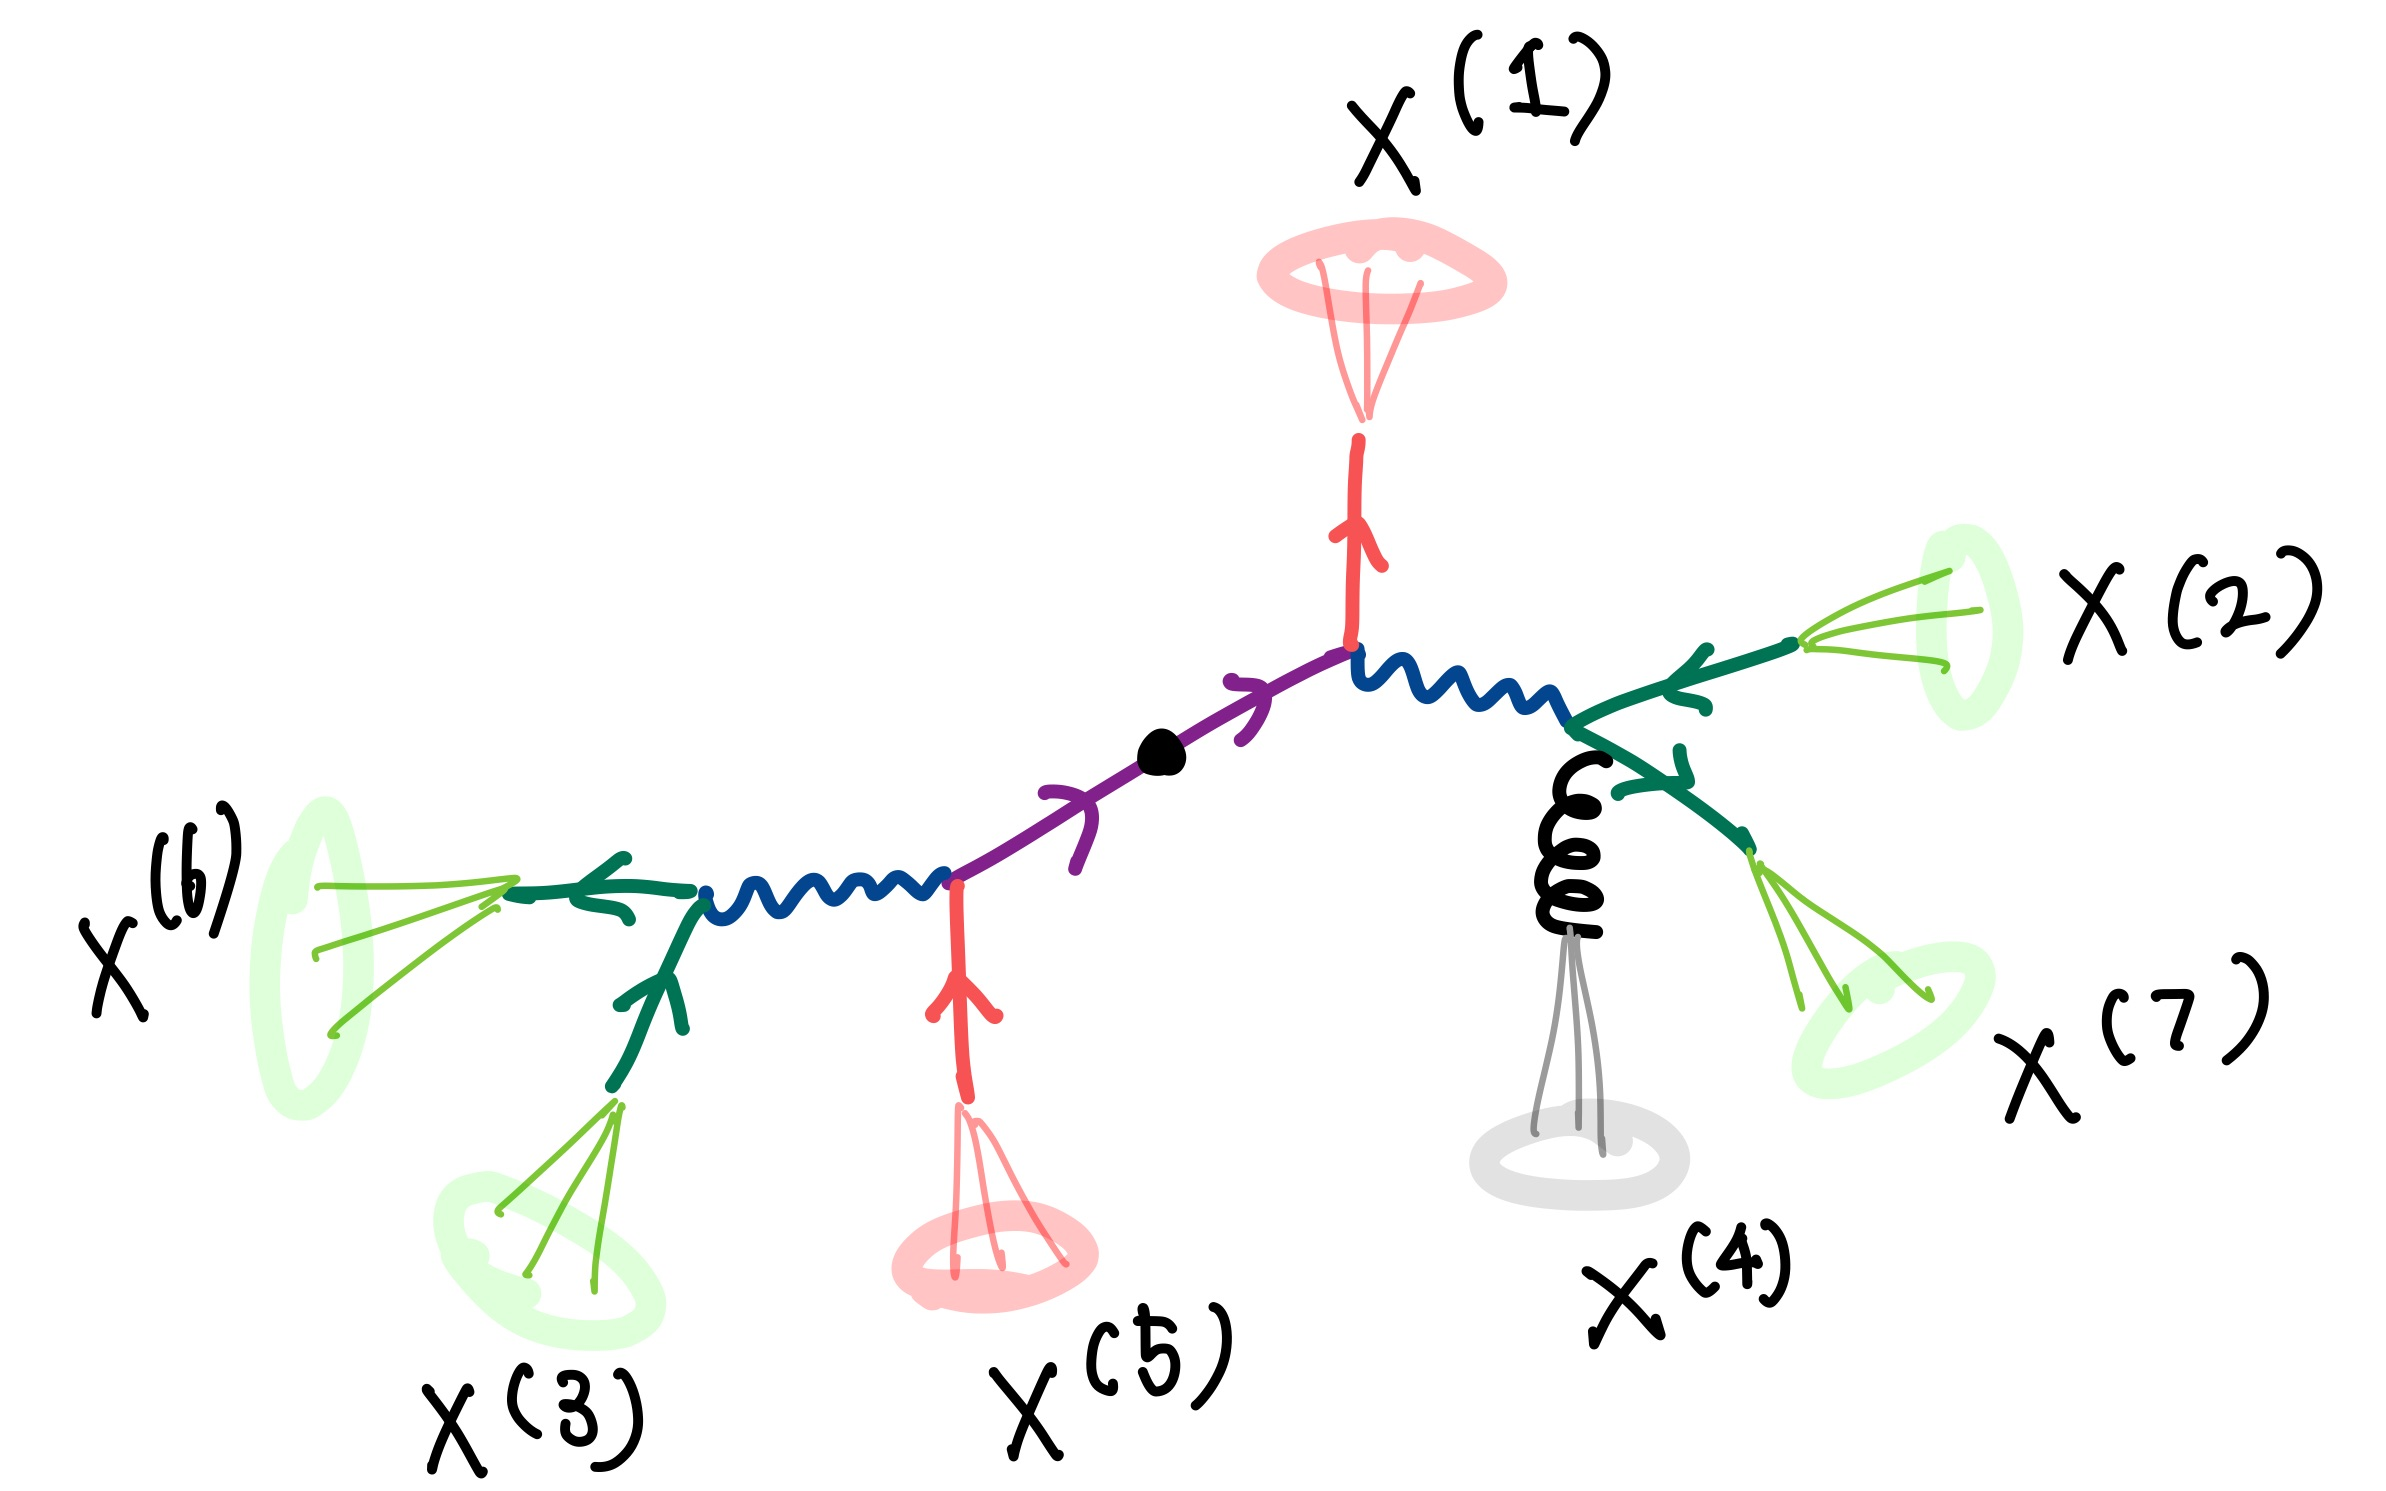
\includegraphics[width=0.3\textwidth]{fig/model-cartoon/saja-input.jpg}
        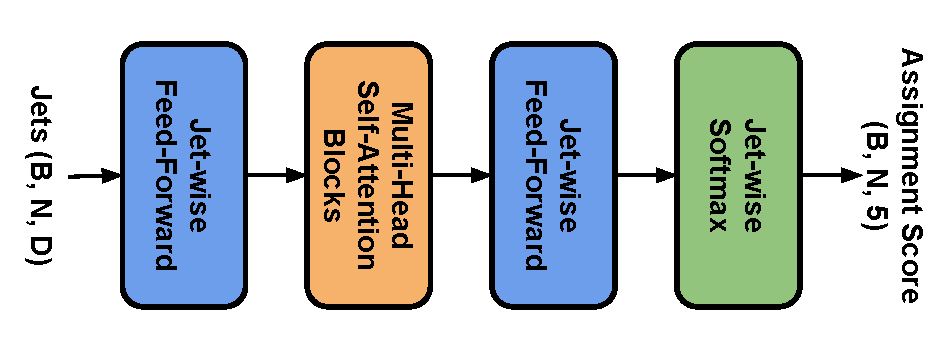
\includegraphics[width=0.3\textwidth]{fig/model-cartoon/model-rot270.pdf}
        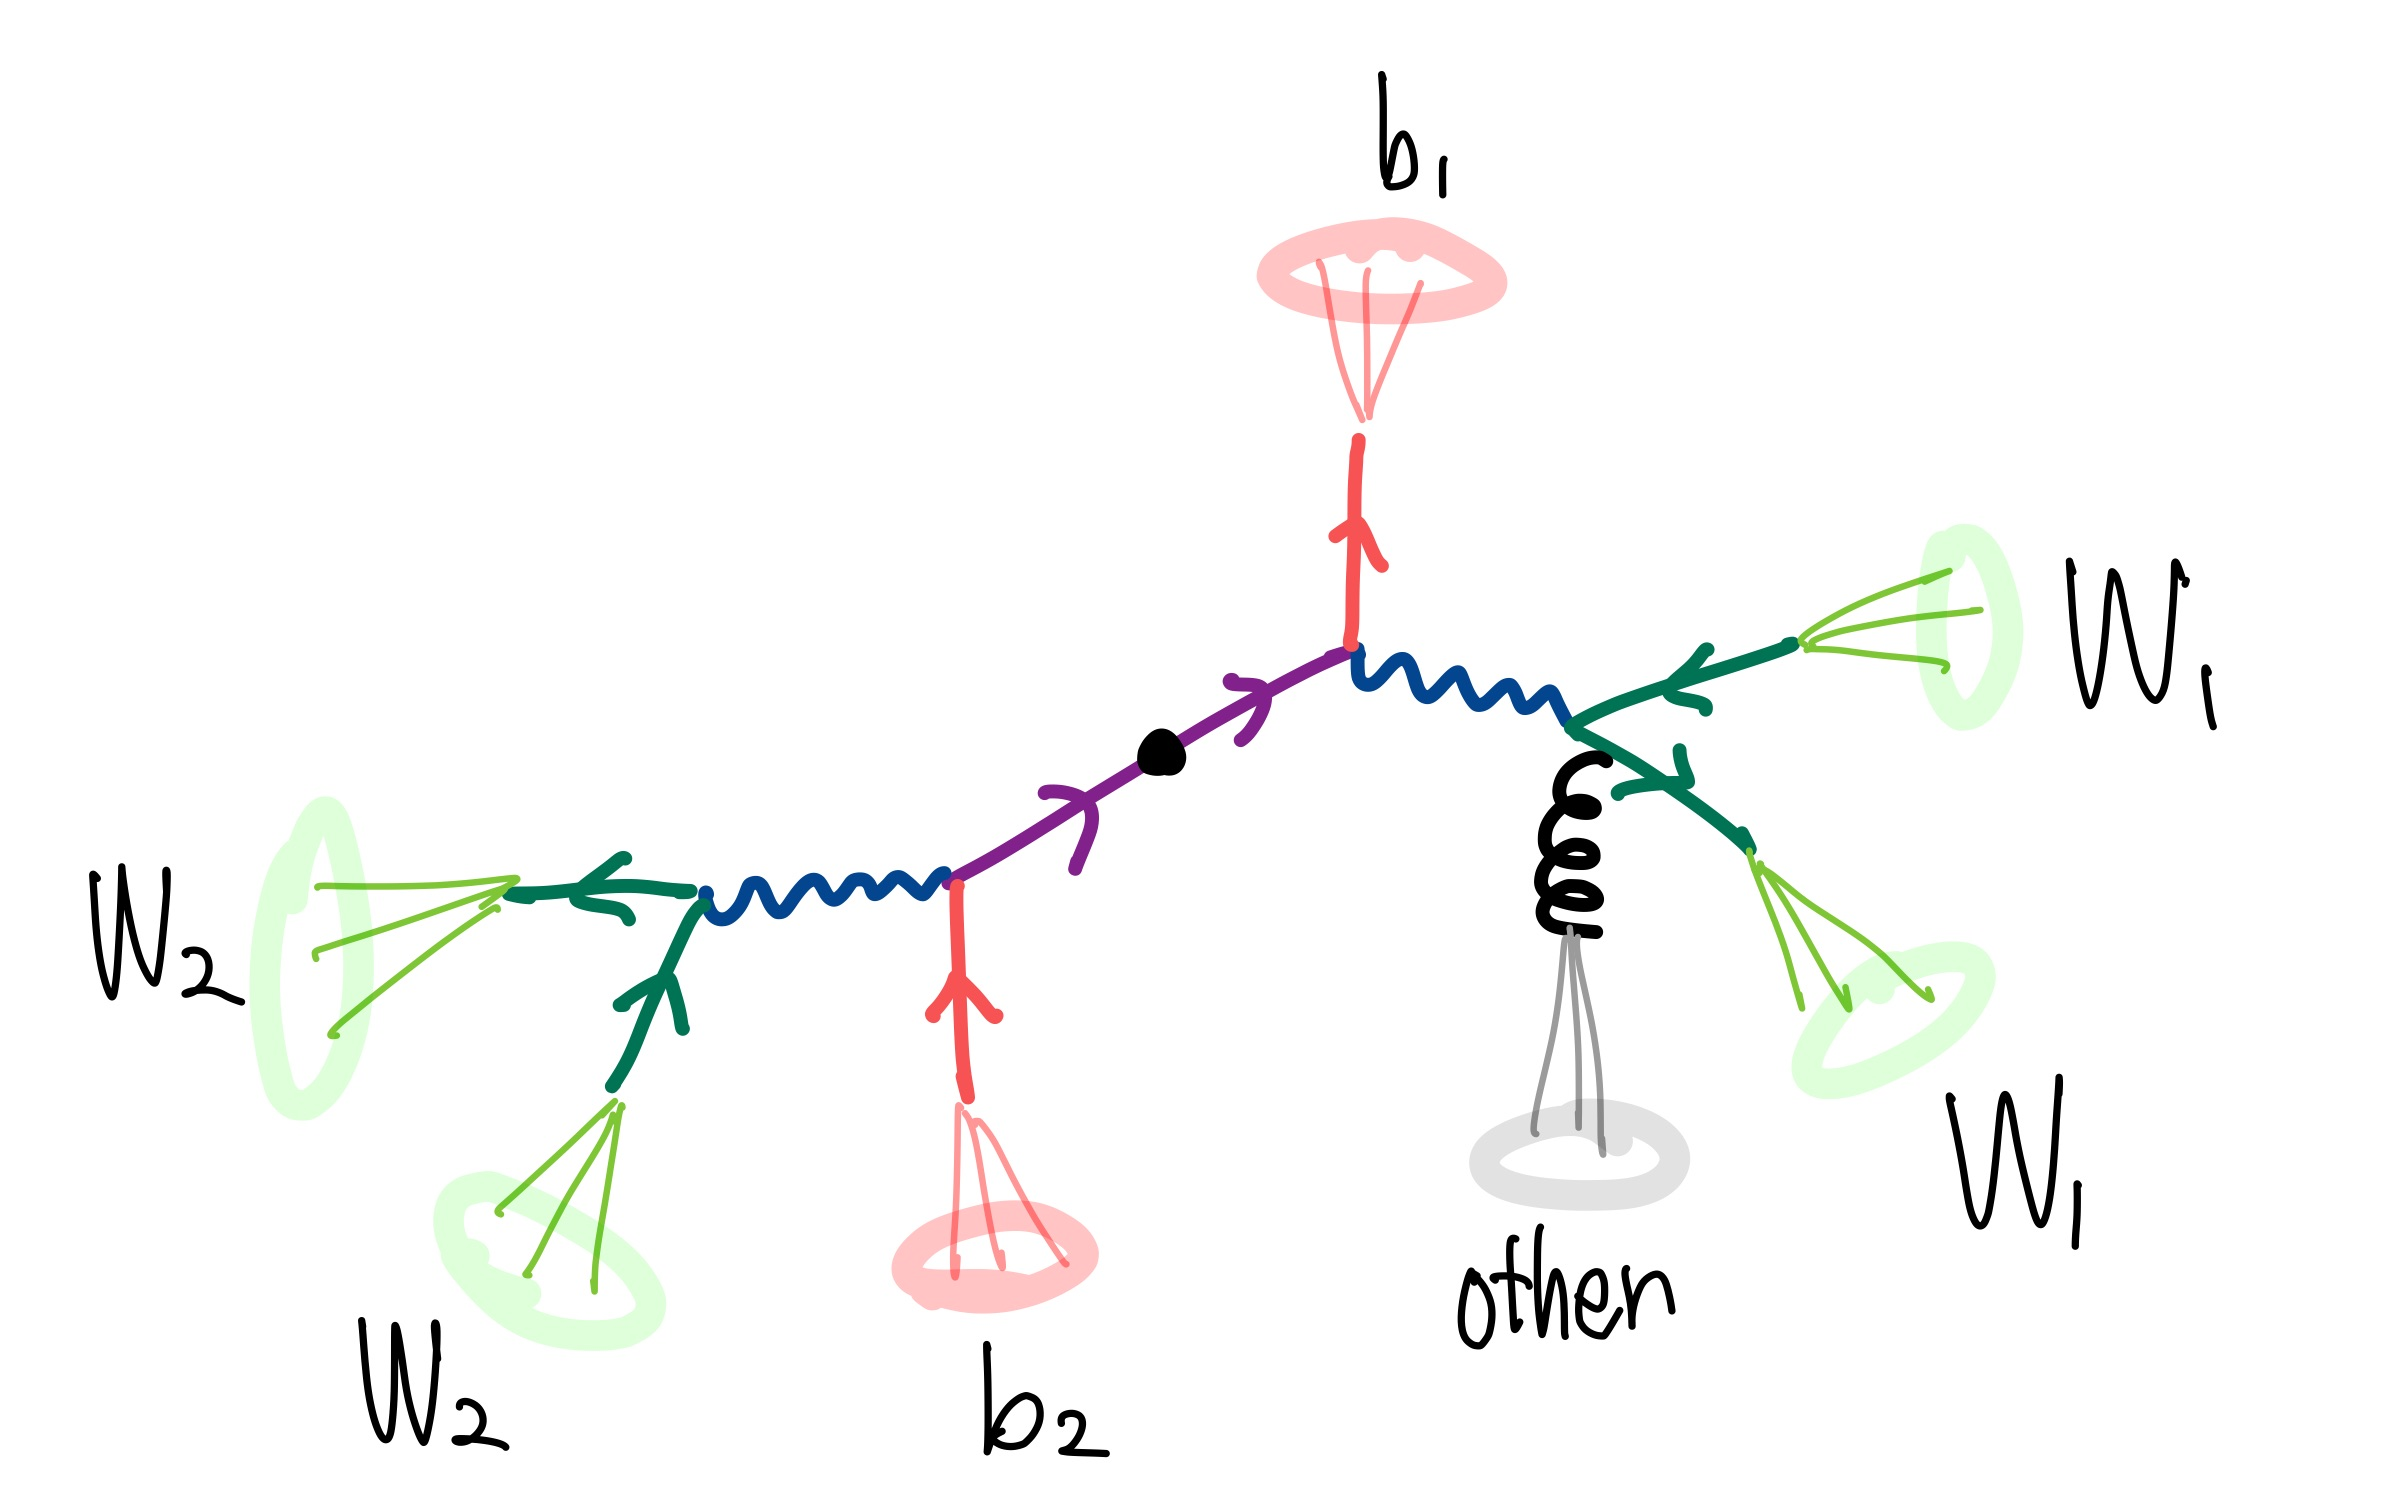
\includegraphics[width=0.3\textwidth]{fig/model-cartoon/saja-output.jpg}
    \end{figure}
\end{frame}

%%%%%%%%%%%%%%%%%%%%%%%%%%%%%%%%%%%%%%%%%%%%%%%%%%%%%%%%%%%%%%%%%%%%%%%%%%%%%%%

\begin{frame}[fragile]{Objective function}
    Since the indices 1 and 2 are arbitrary, the general objective function cannot be used here. \break
    Therefore, a new cross-entropy based objective function is introduced.
    \begin{gather*}
        J(\theta) = \frac{1}{N} \sum_{j=1}^{N}[\min{(\pi_{12}^{(j)}, \pi_{21}^{(j)})} + y_{ \textrm{other} }^{(j)} \log{\hat{y}_{\textrm{other}}^{(j)}}],
        \intertext{where}
        \pi_{\alpha\beta}^{(j)} = -\left[
            y_{b}^{(j)} \log{\hat{y}_{b_{\alpha}}^{(j)}}
            + y_{\bar{b}}^{(j)} \log{\hat{y}_{b_{\beta}}^{(j)}} 
            + y_{W^{+}}^{(j)} \log{\hat{y}_{W_{\alpha}}^{(j)}}
            + y_{W^{-}}^{(j)} \log{\hat{y}_{W_{\beta}}^{(j)}}
            \right].
    \end{gather*}
    
    $\Rightarrow$ A deep learning model of any architecture can become
    a \underline{\textbf{zero-permutation jet-parton assignment model}}
    if it is fit by minimizing the above objective function.
\end{frame}

%%%%%%%%%%%%%%%%%%%%%%%%%%%%%%%%%%%%%%%%%%%%%%%%%%%%%%%%%%%%%%%%%%%%%%%%%%%%%%%
\begin{frame}[fragile]{Self-Attention based Model Architecture}
  \begin{itemize}
    \item[$\bullet$]
        The model implementation is based on \textsc{Transformer}, which is
        the neural machine translation model and features \underline{\textbf{self-attention}}.
        \href{https://arxiv.org/abs/1706.03762}{[A. Vaswani, arXiv:1706.03762]}
    \item[$\bullet$]
        Self-attention performs a weight sum of the elements (vectors) of
        the input set, where the weight matrix is also computed from the elements.
      \begin{itemize}
        \item Sentence = a set of words
        \item Image = a set of pixels
        \item Event = a set of jets
      \end{itemize}
    \item[$\bullet$] Self-attention based model can learn the dependency between elements.
  \end{itemize}
\end{frame}

%%%%%%%%%%%%%%%%%%%%%%%%%%%%%%%%%%%%%%%%%%%%%%%%%%%%%%%%%%%%%%%%%%%%%%%%%%%%%%%
\begin{frame}[fragile]{Self-Attention based Model Architecture \saja}
    \begin{figure}
        \centering
        \begin{subfigure}[t]{0.3\textwidth}
            \centering
            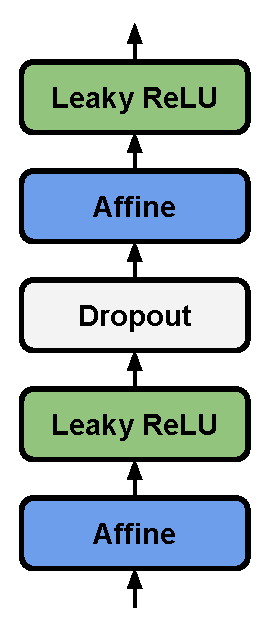
\includegraphics[width=\textwidth, height=4cm, keepaspectratio]{fig/model/jet-wise-feed-forward.pdf}
            \caption{Jet-wise feed-forward network}
        \end{subfigure}
        \hfill  
        \begin{subfigure}[t]{0.3\textwidth}
            \centering
            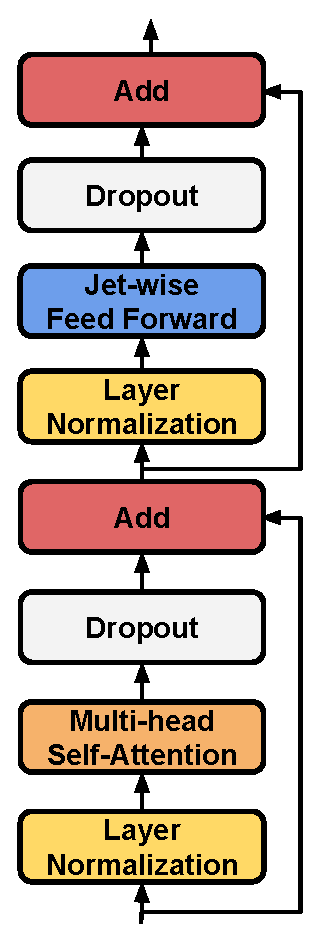
\includegraphics[width=\textwidth, height=5cm, keepaspectratio]{fig/model/attention-block.pdf}
            \caption{Multi-head self-attention block}
        \end{subfigure}
        \hfill
        \begin{subfigure}[t]{0.3\textwidth}
            \centering
            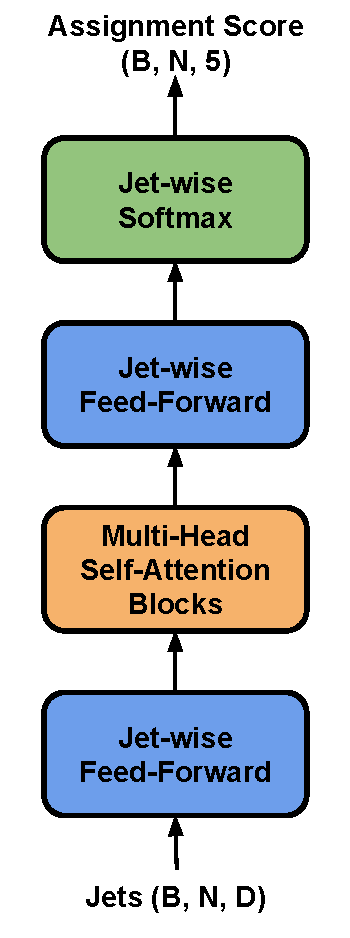
\includegraphics[width=\textwidth, height=4cm, keepaspectratio]{fig/model/model.pdf}
            \caption{\saja, Jet-parton assignment model}
        \end{subfigure}
      \hfill
    \end{figure}

    {\footnotesize \saja, is invariant to the order of jets and this permutation
     invariant property can be used to peek inside the black box of \saja,
     with Monte Carlo information.}
\end{frame}

%%%%%%%%%%%%%%%%%%%%%%%%%%%%%%%%%%%%%%%%%%%%%%%%%%%%%%%%%%%%%%%%%%%%%%%%%%%%%%%

\begin{frame}[fragile]{Simulation}
    \begin{block}{$\blacksquare$ Generation}
        \smallskip
        \begin{itemize}
          \item pp collision with $\sqrt{s}=13\,\TeV$ using $\textsc{MadGraph5\_aMC@NLO}$ and ${\PYTHIA}8$
            \item Fully hadronic \ttbar with up to two additional jets at NLO, $m_{t}=172.5\,\GeV$
            \item QCD multijet at LO.
        \end{itemize}
    \end{block}
    \medskip
    \begin{block}{$\blacksquare$ Detector response}
        \smallskip
        \begin{itemize}
            \item \textsc{Delphes3}
            \item CMS-like detector
        \end{itemize}
    \end{block}
    \begin{block}{$\blacksquare$ Jet Finding}
        \smallskip
        \begin{itemize}
            \item \textsc{FastJet3}
            \item anti-$k_{T}$ algorithm with R=0.4
        \end{itemize}
    \end{block}
\end{frame}

%%%%%%%%%%%%%%%%%%%%%%%%%%%%%%%%%%%%%%%%%%%%%%%%%%%%%%%%%%%%%%%%%%%%%%%%%%%%%%%
\begin{frame}[fragile]{Selection}
  Selection follows the trigger selection used in the CMS \ttbar all-jets analysis.
  {\scriptsize \href{https://link.springer.com/article/10.1140\%2Fepjc\%2Fs10052-019-6788-2}{[CMS, Eur. Phys. J. C 79 (2019) 313]}}.

  \begin{columns}[T,onlytextwidth]
    \column{\textwidth}
    \begin{block}{$\blacksquare$ Jet}
      \begin{itemize}
        \item \( \pt > 30\,\GeV \)
        \item \( \abs{\eta} < 2.4 \)
        \item[+]  b-tag: true/fake based on the efficiency for b quark and
                  misidentification rates for gluon, light quark jets and c-jets.
      \end{itemize}
    \end{block}
    
    \begin{block}{$\blacksquare$ Event}
        \begin{itemize}
            \item $N_{\text{jet}} \ge 6$
            \item At least one b-tagged jet of the six most energetic jets
            \item ${\pt}(\text{jet}_{6}) > 40\,\GeV$
            \item $H_{T} \equiv \sum_{\textrm{jet}} {\pt} > 450\,\GeV$
        \end{itemize}
    \end{block}
  \end{columns}
\end{frame}

%%%%%%%%%%%%%%%%%%%%%%%%%%%%%%%%%%%%%%%%%%%%%%%%%%%%%%%%%%%%%%%%%%%%%%%%%%%%%%%
\begin{frame}[fragile]{Jet-Parton Matching}
  After the event selection, only about 20\% of \ttbar events satisfy the
  following jet-parton matching condition and are called \textbf{matched}.
  $$\Delta R(\text{jet}, \text{parton}) = \sqrt{\Delta\eta^{2}+\Delta\phi^{2}} < 0.3$$
  Only the matched \ttbar events are used to train the DL model.
  \begin{columns}[T,onlytextwidth]
    \column{0.48\textwidth}
    \begin{figure}
      \centering
      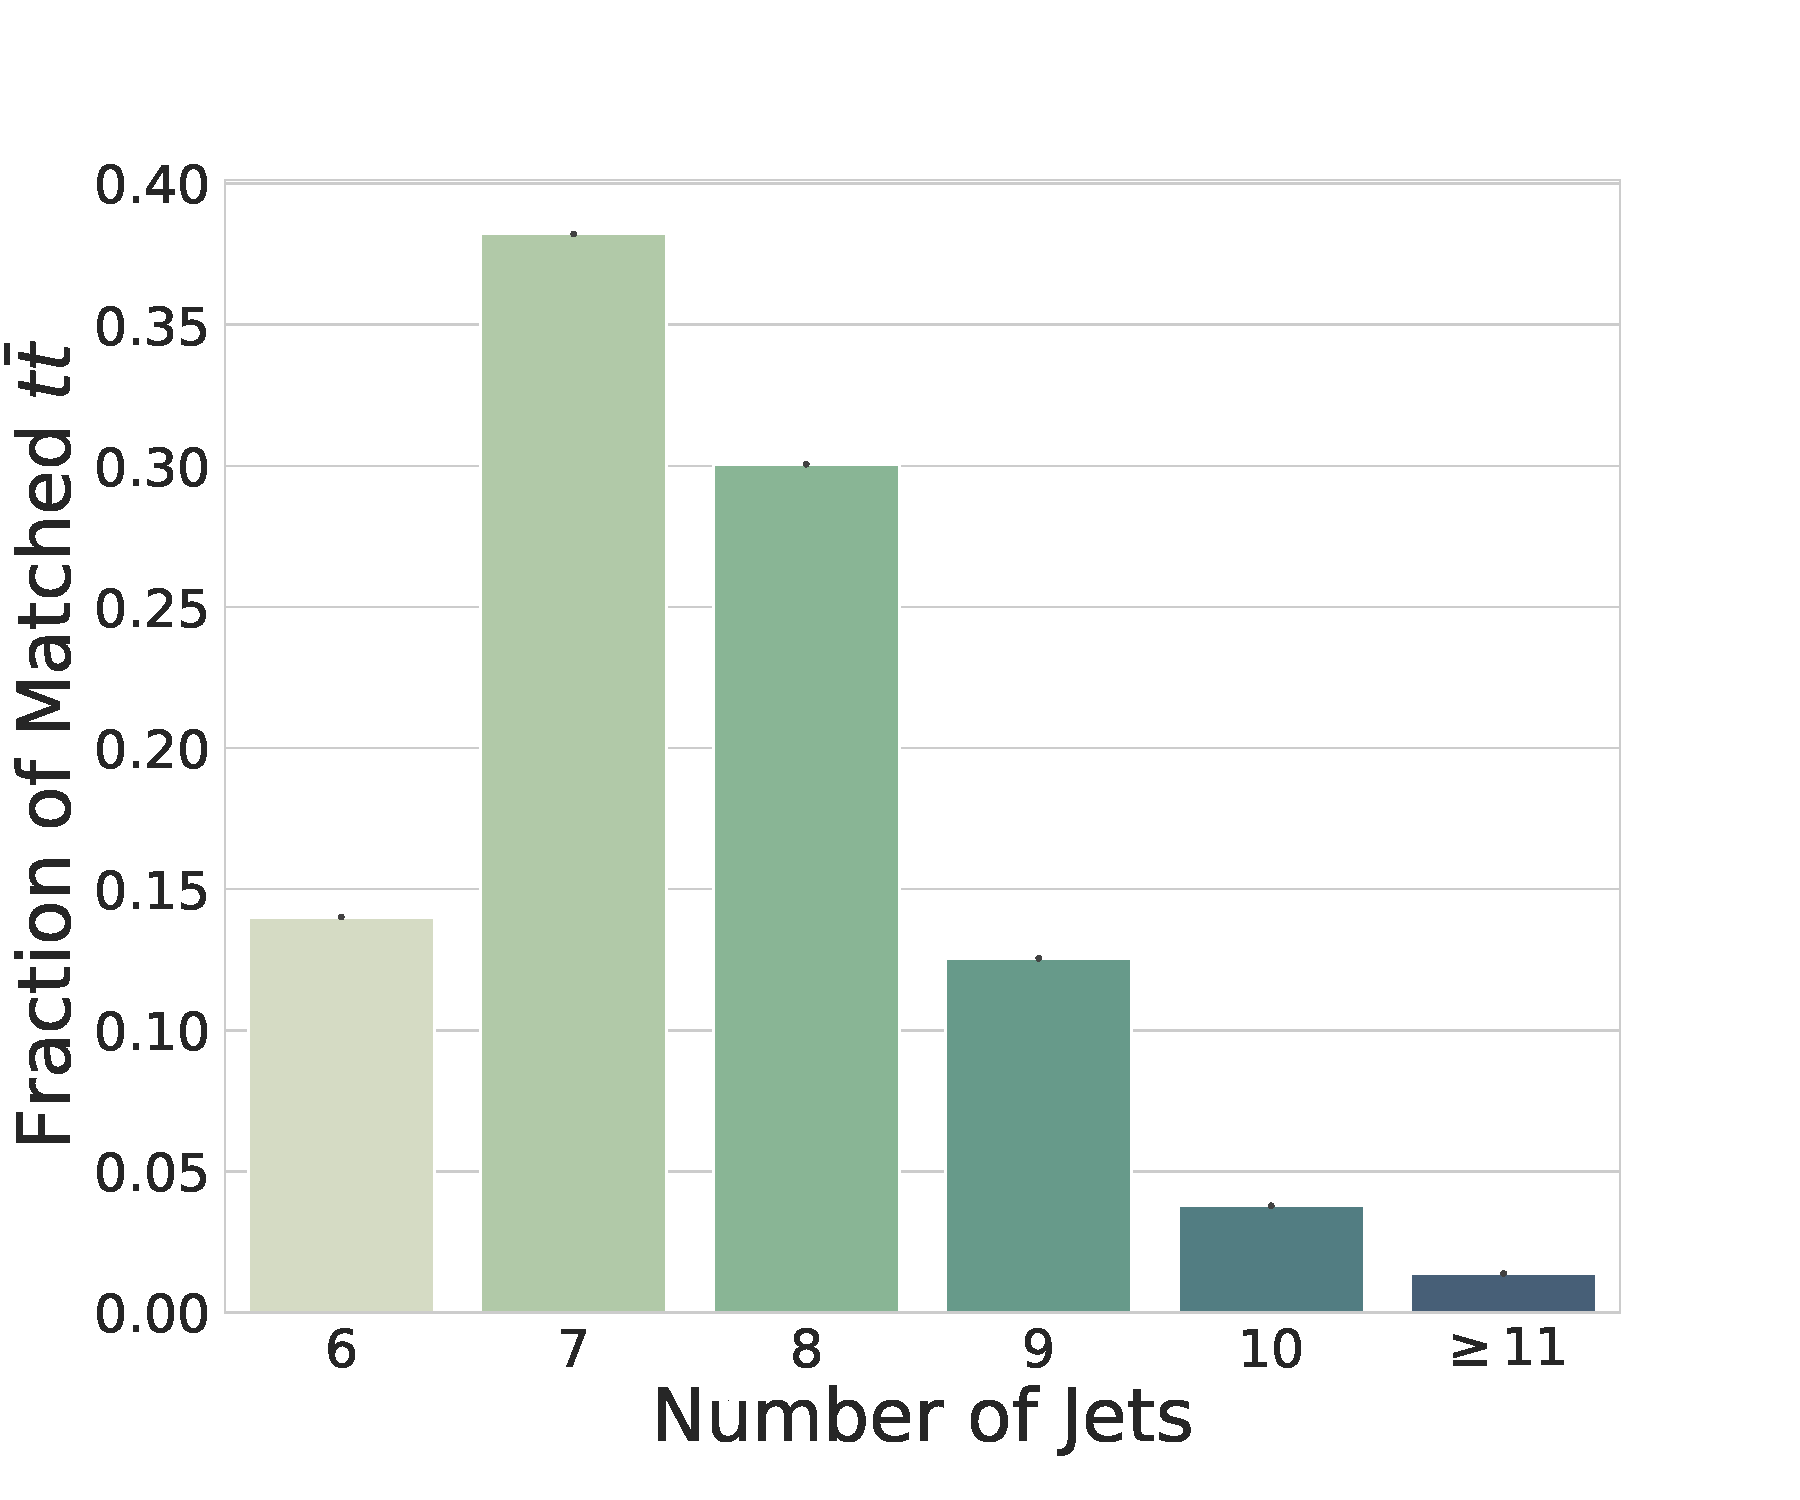
\includegraphics[width=0.8\textwidth]{fig/jet-parton-matching/num-jets.pdf}
      \caption{The distribution of the number of jets in the matched \ttbar events}
    \end{figure}
    \column{0.48\textwidth}
    \begin{figure}
      \centering
      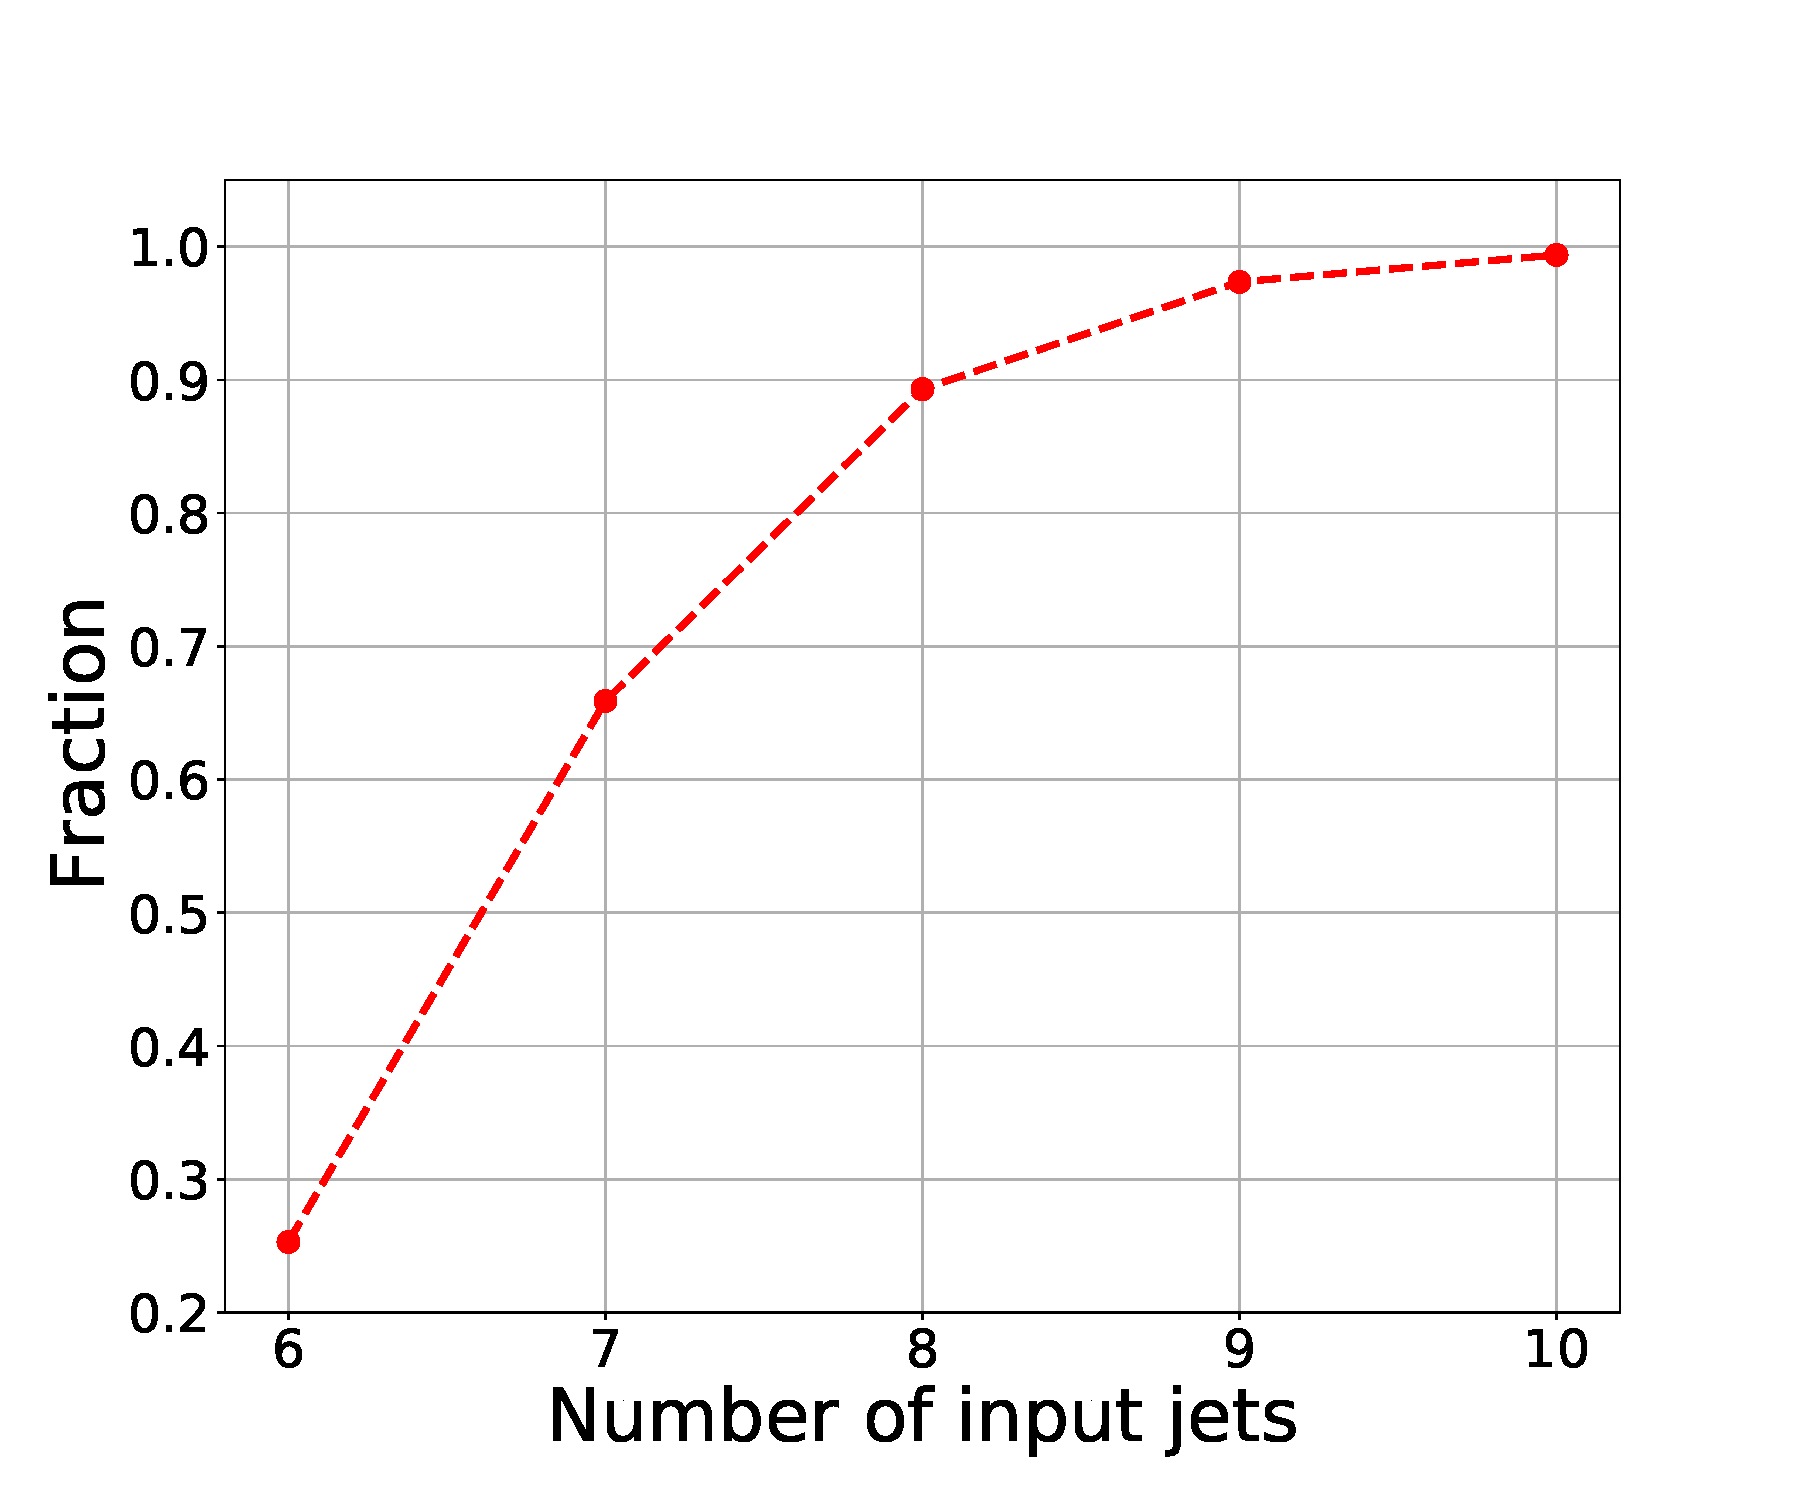
\includegraphics[width=0.8\textwidth]{fig/jet-parton-matching/frac-vs-num-jets.pdf}
      \caption{The fraction of matched \ttbar events, where all partons can be matched with the most energetic $N$ jets.}
      %\label{fig:my_label}
    \end{figure}
  \end{columns}
\end{frame}


%%%%%%%%%%%%%%%%%%%%%%%%%%%%%%%%%%%%%%%%%%%%%%%%%%%%%%%%%%%%%%%%%%%%%%%%%%%%%%%
\begin{frame}[fragile]{Training Dataset}
  \begin{block}{$\blacksquare$ Event}
    \smallskip
    All jets in the event are used as input to the model.
    
    For simplicity, the jet is high level reconstructed variables.
    $$\footnotesize ({\pt}, \eta, \phi, \frac{p_{T}}{H_{T}}, \text{b-tag})$$
  \end{block}
  \begin{block}{$\blacksquare$ Jet Shape}
    %\smallskip
    Gluon-initiated jets should always be assigned to $'\text{other}'$.
    So the effect of the following jet shape variables is studied.
    \href{https://arxiv.org/abs/1409.3072}{[CMS, arXiv:1409.3072]}
    \begin{itemize}
      \item {\footnotesize ${\pt}D=\frac{ \sum_{i} p_{T,i}^{2} }{ \sum_{i} p_{T,i} }$}
      \item {\footnotesize Major and minor axes of the jet axis in $\eta-\phi$ space}
      \item {\footnotesize Charged hadron, neutral hadron, electrons, muon, and photon multiplicities}
    \end{itemize}
  \end{block}
  \begin{block}{$\blacksquare$ Pre-processing}
      %\smallskip
      {\footnotesize All features except b-tag is scaled to [0, 1]
      through min-max scaling $x'=\frac{x-\min({x})}{\max({x})-\min({x})}$}
  \end{block}
\end{frame}

%%%%%%%%%%%%%%%%%%%%%%%%%%%%%%%%%%%%%%%%%%%%%%%%%%%%%%%%%%%%%%%%%%%%%%%%%%%%%%%
\begin{frame}[fragile]{Predictive Entropy}
  \begin{columns}[T,onlytextwidth]
    \column{0.65\textwidth}
    %If any of the predictions for the jets in the event is also wrong, the jet-parton assignment is wrong.\\

    $\bullet$ To suppress poor jet-parton assignments, the DL model uncertainty is studied.\\
    
    \medskip
    
    $\bullet$ The \textbf{predictive entropy} quantifies the uncertainty in the prediction of the classifier.
    \begin{equation*}
        H[\hat{Y}] = \frac{1}{N} \sum_{j=1}^{N} [ -\sum_{c \in \textrm{partons} } \hat{y}_{c}^{(j)} \log \hat{y}_{c}^{(j)} ]
    \end{equation*}
    
    $\bullet$ When the jet-parton assignment with the predictive entropy higher than the threshold, the event is not selected.

    + The uncertainty is also used to detect out-of-distribution test data (corresponding to QCD in this study).
    \column{0.3\textwidth}
    \begin{figure}
      \centering
      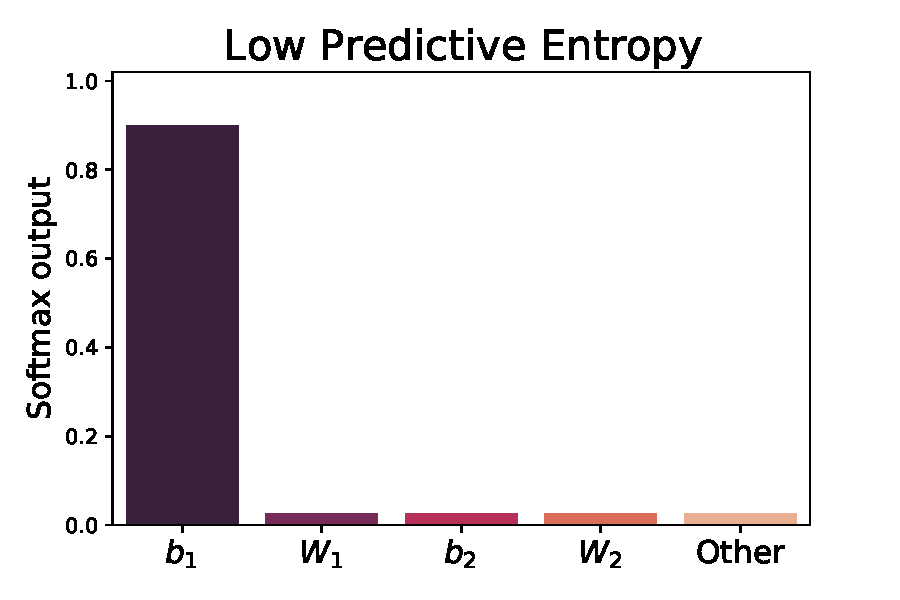
\includegraphics[width=\textwidth]{fig/entropy-example/entropy-low.pdf}
      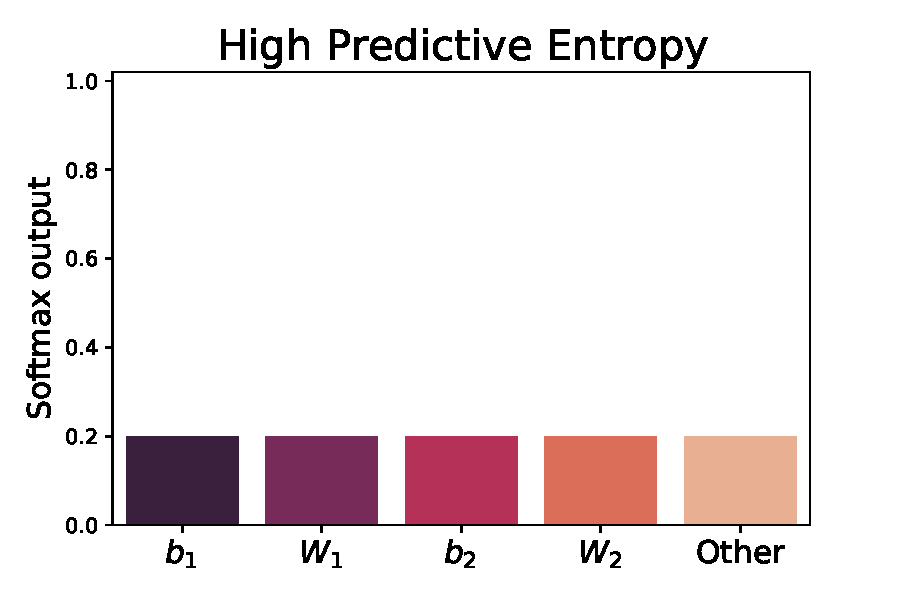
\includegraphics[width=\textwidth]{fig/entropy-example/entropy-high.pdf}
      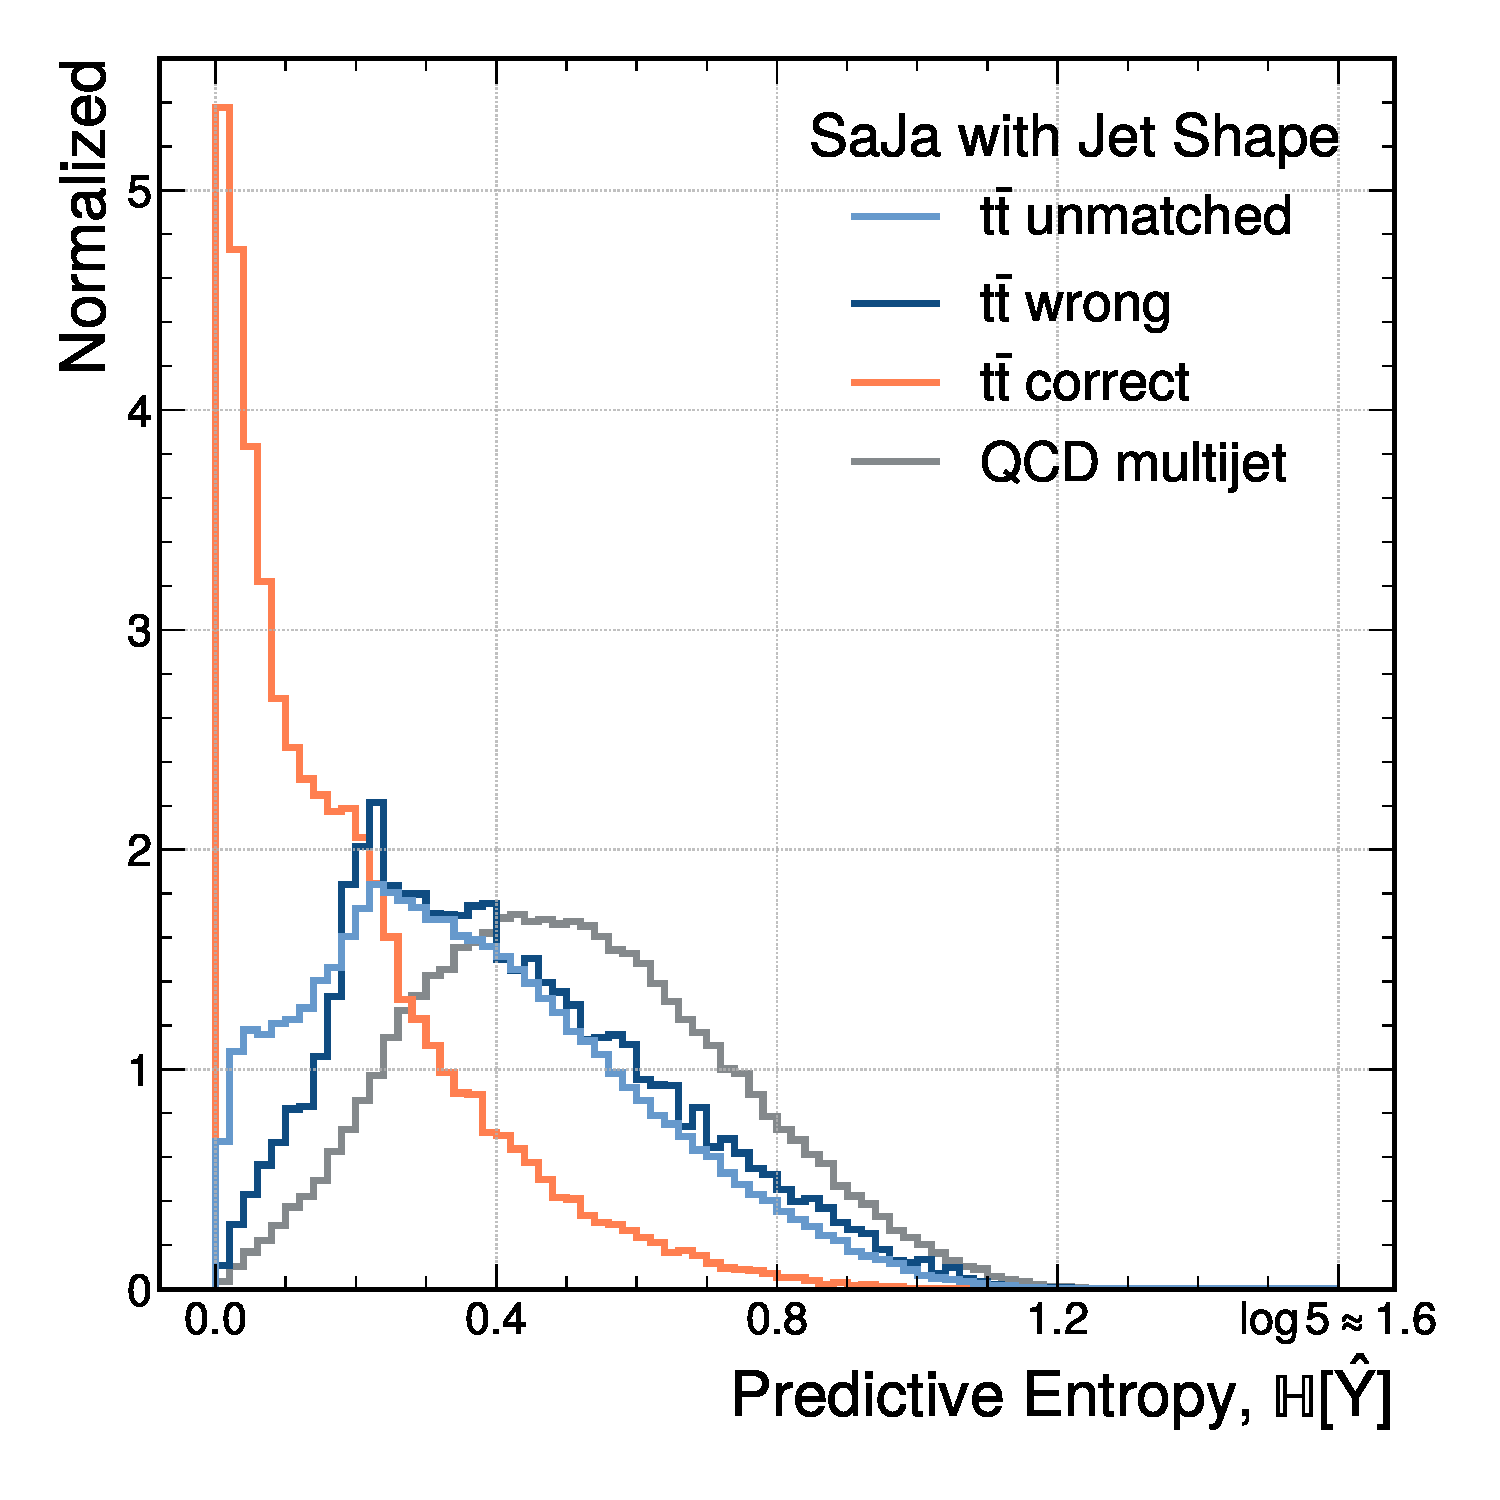
\includegraphics[width=\textwidth]{fig/entropy/entropy-with-jet-shape.pdf}
    \end{figure}
  \end{columns}
  
\end{frame}


%%%%%%%%%%%%%%%%%%%%%%%%%%%%%%%%%%%%%%%%%%%%%%%%%%%%%%%%%%%%%%%%%%%%%%%%%%%%%%%
\begin{frame}[fragile]{Performance}
  \begin{columns}
    \column{0.55\textwidth}
      \begin{itemize}
        \item
            The assignment performance is visualized as ROC-like curves drawn by
            varying the threshold value for the predictive entropy of \saja or
            the likelihood of \textsc{KLFitter}.
        \item
            \saja shows more powerful performance than \textsc{KLFitter}.
        \item
            Predictive entropy not only reduces poor jet-parton assignments but
            also helps reduce unmatched \ttbar and QCD multijet events without
            additional training process.
        \item
            Jet shape increases the fraction of correct assignment.
      \end{itemize} 
      
    \column{0.37\textwidth}
      \begin{figure}
        \centering
        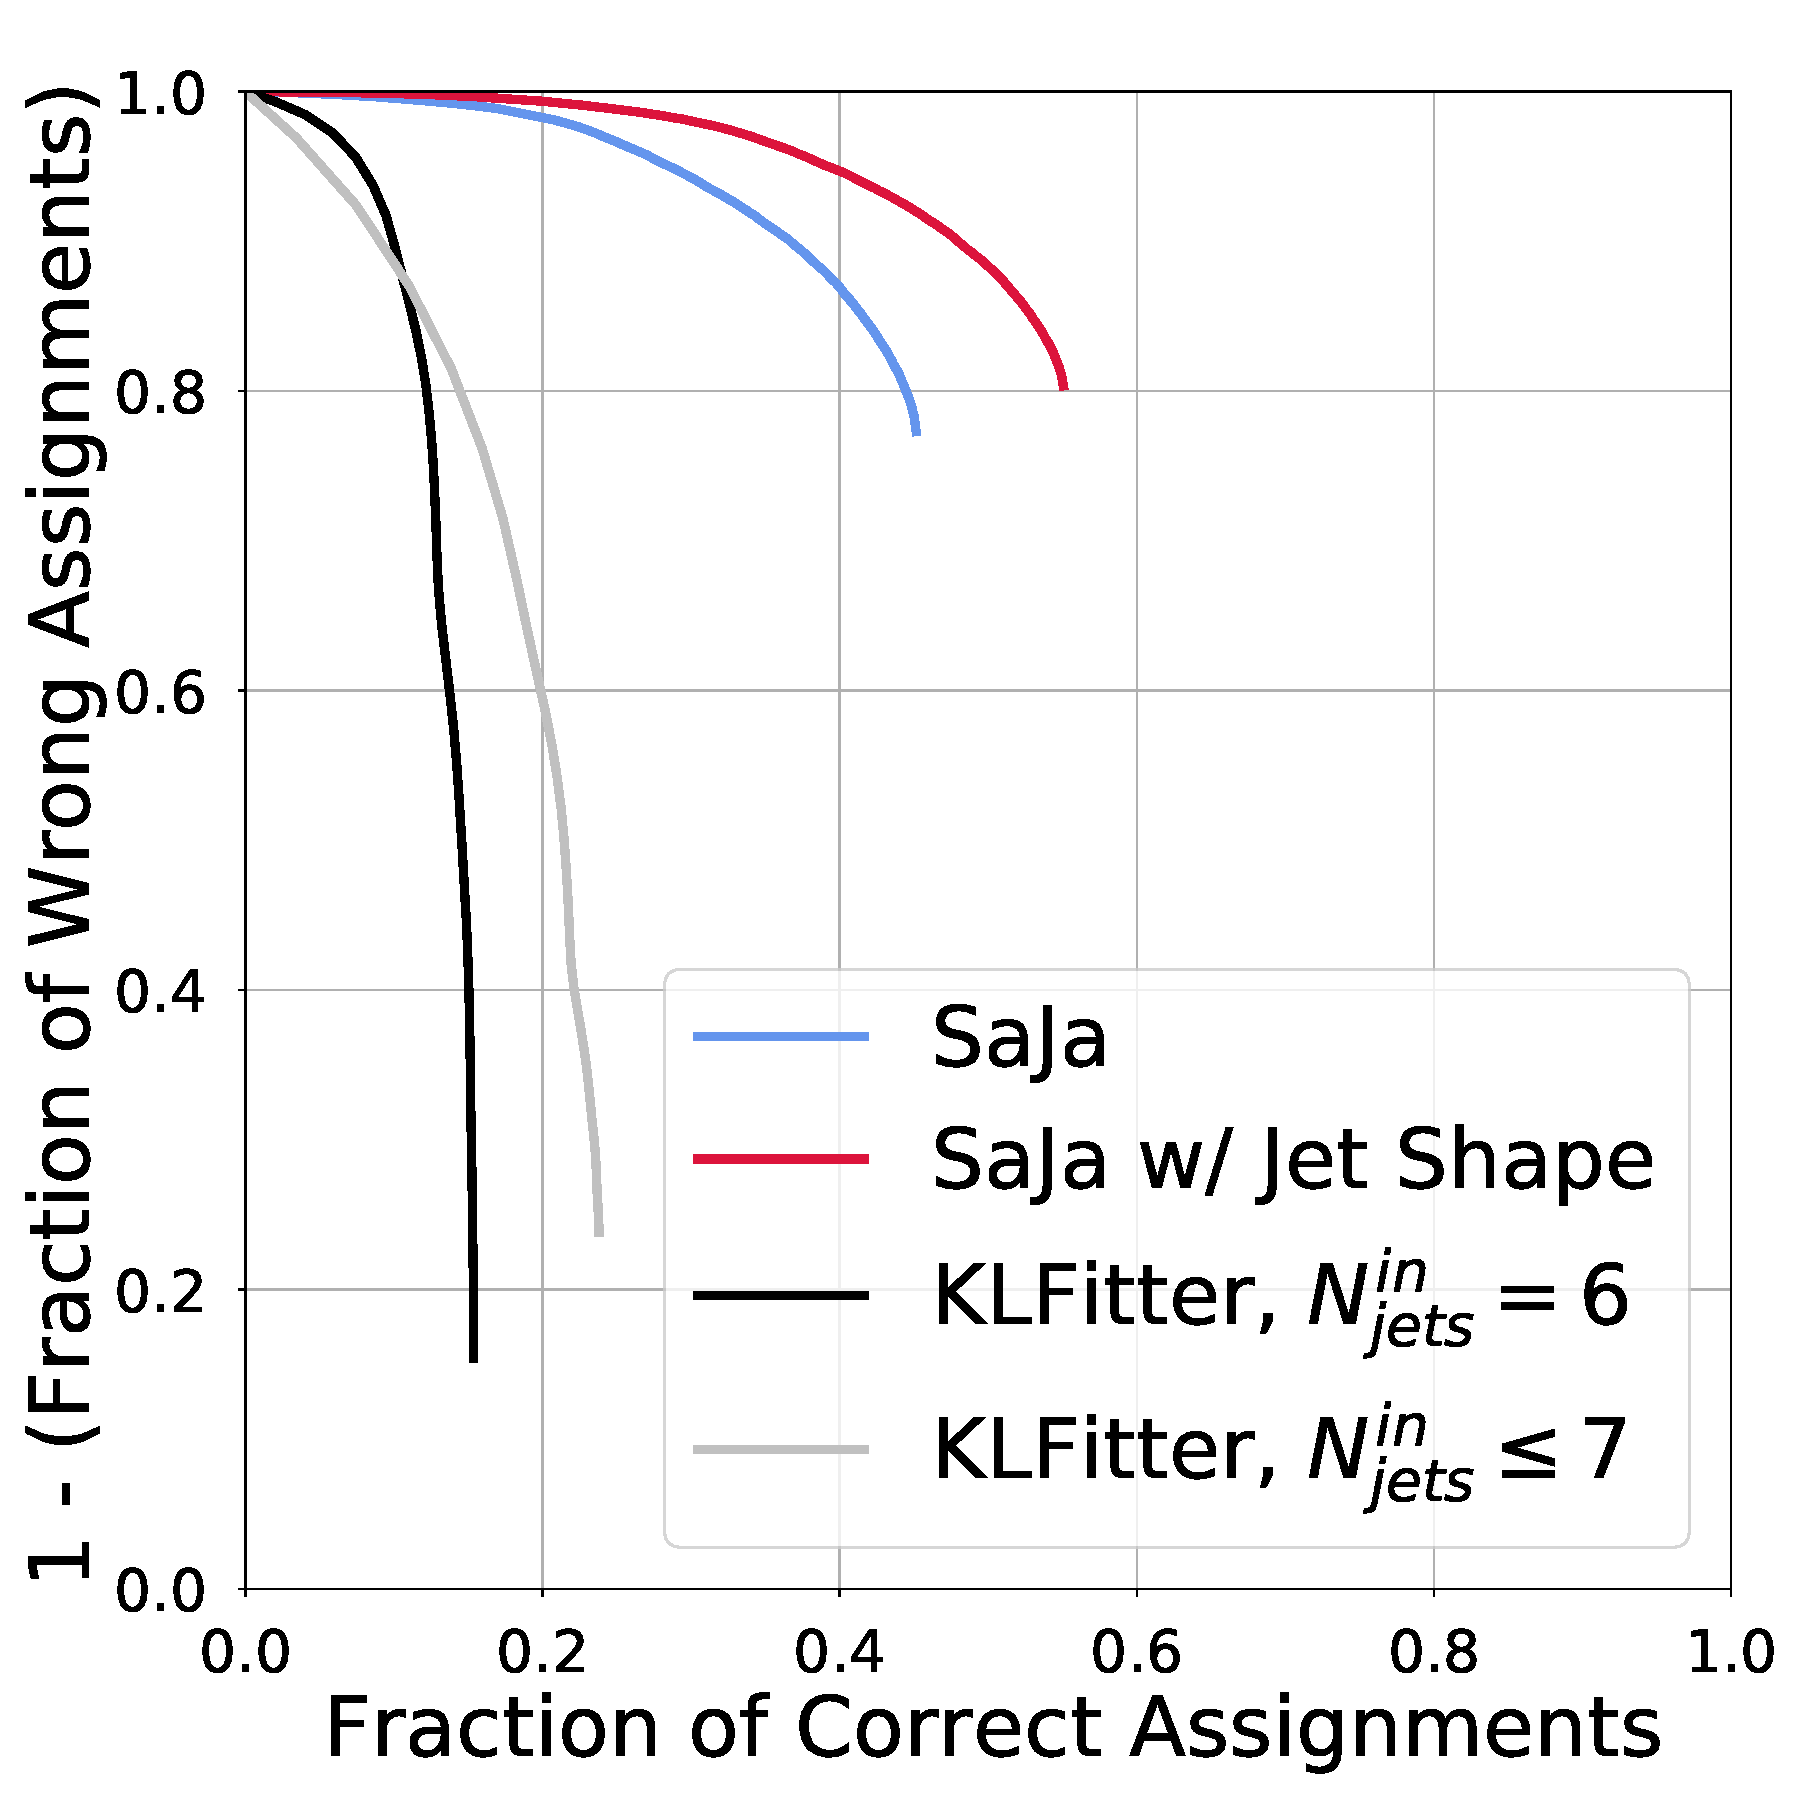
\includegraphics[height=0.32\textheight]{fig/roc/roc_wrong-rej_vs_correct.pdf}
        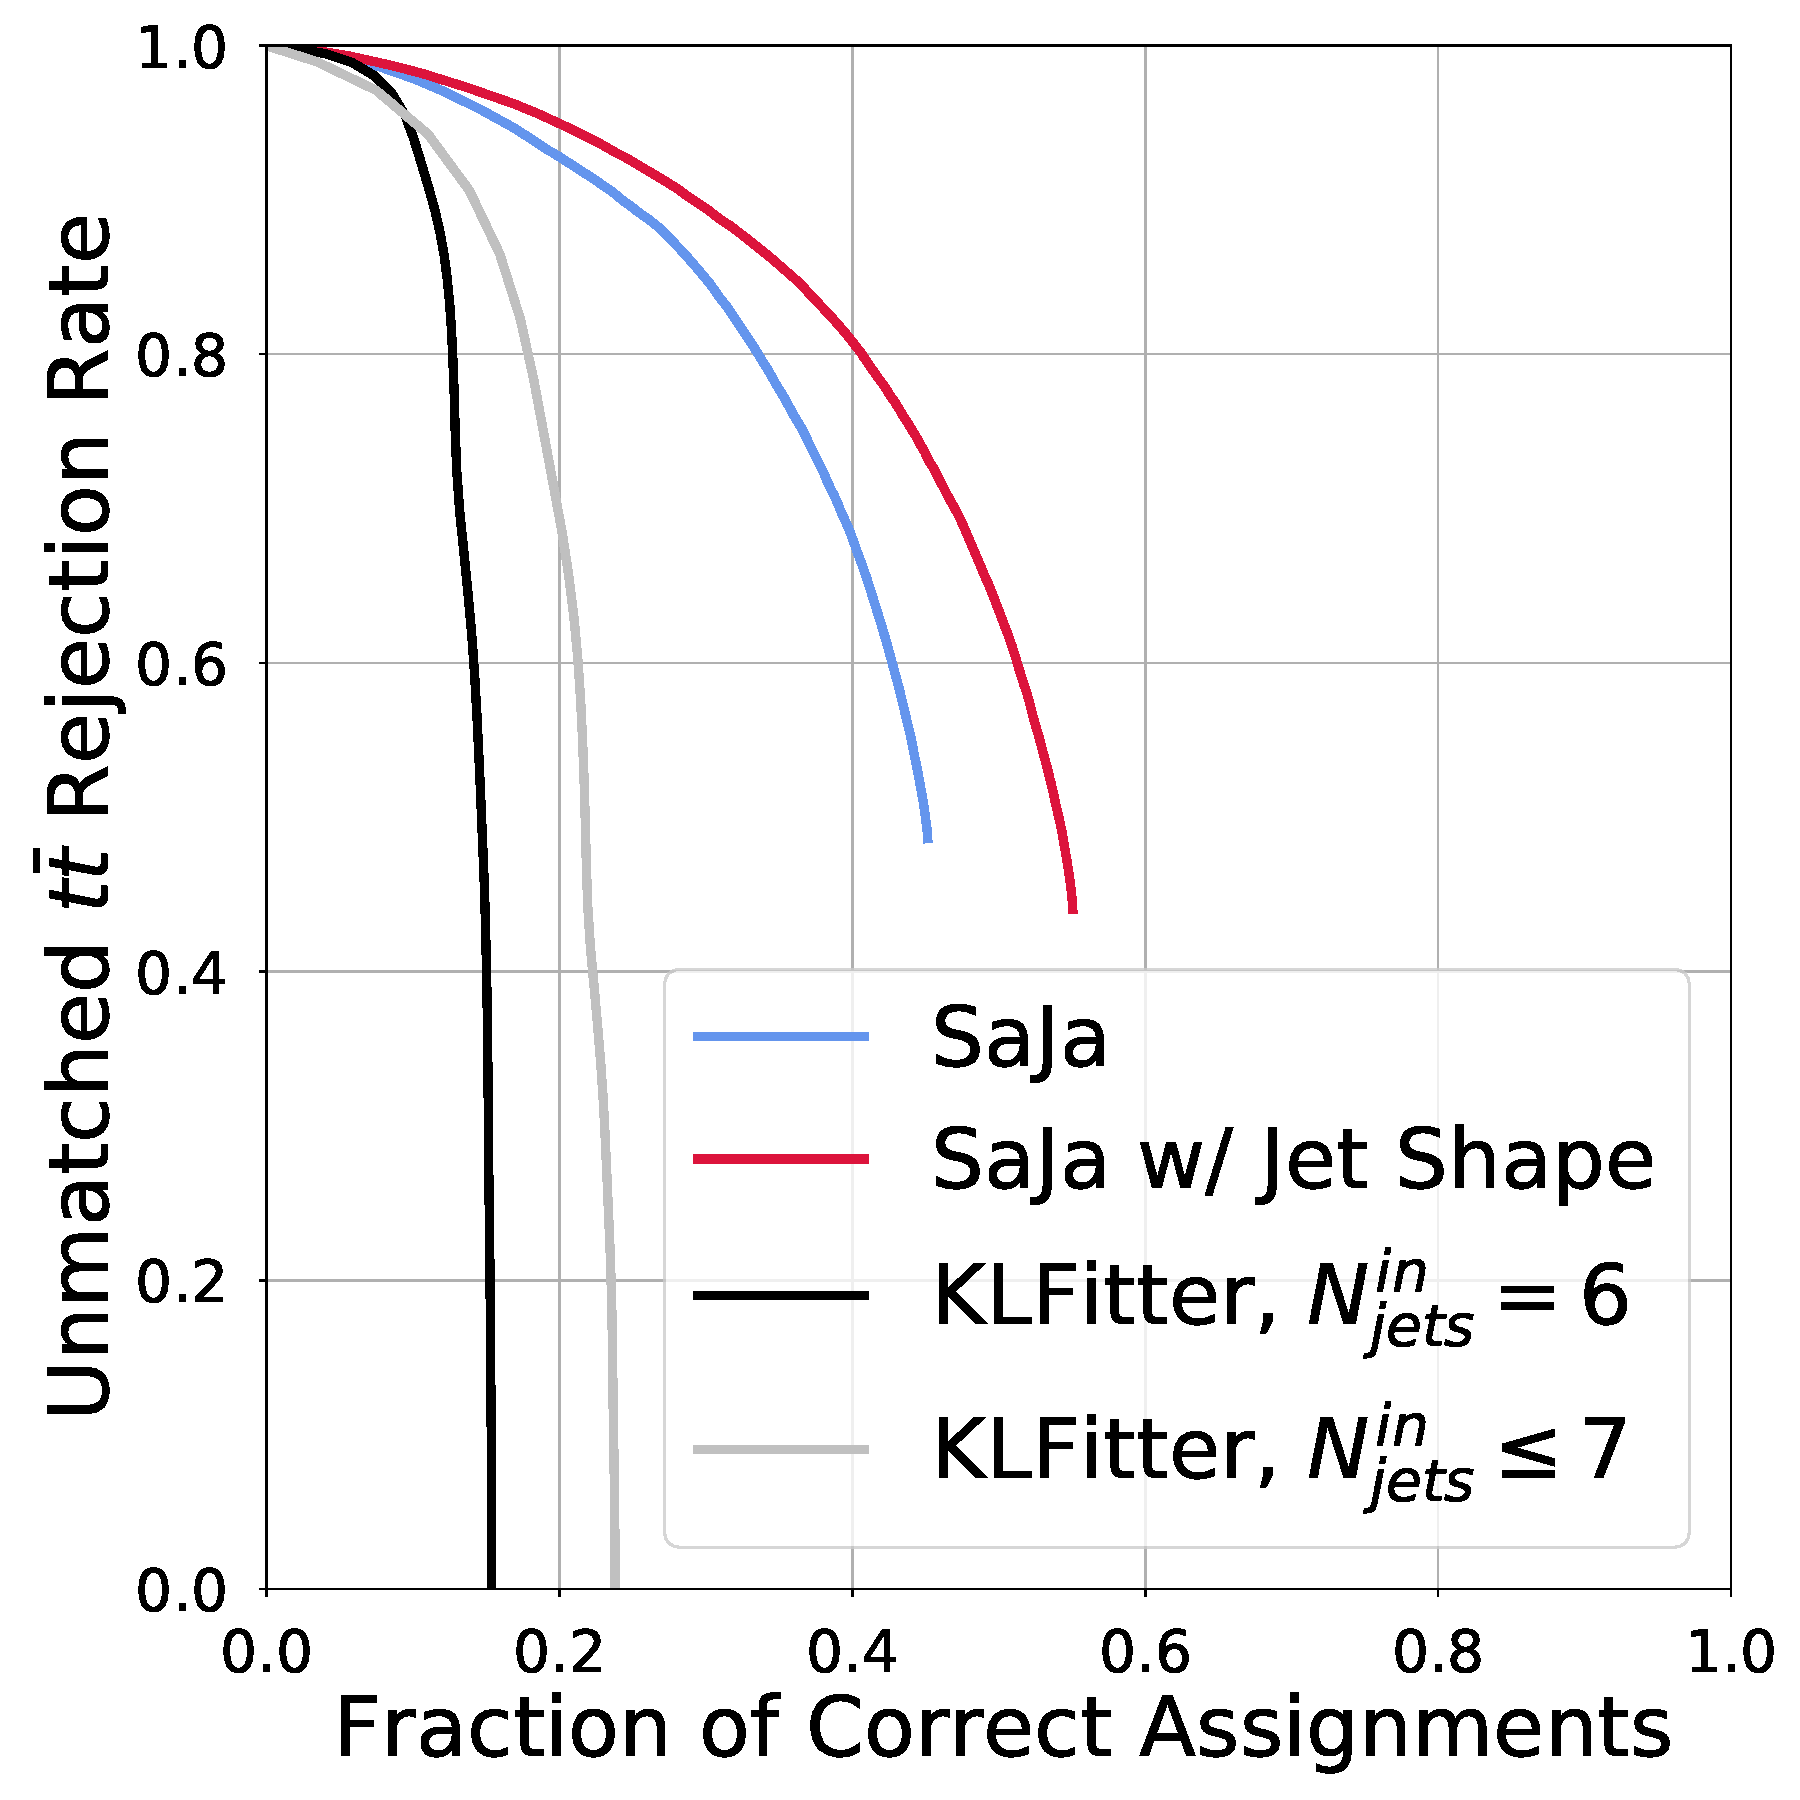
\includegraphics[height=0.32\textheight]{fig/roc/roc_unmathed-rej_vs_correct.pdf}
        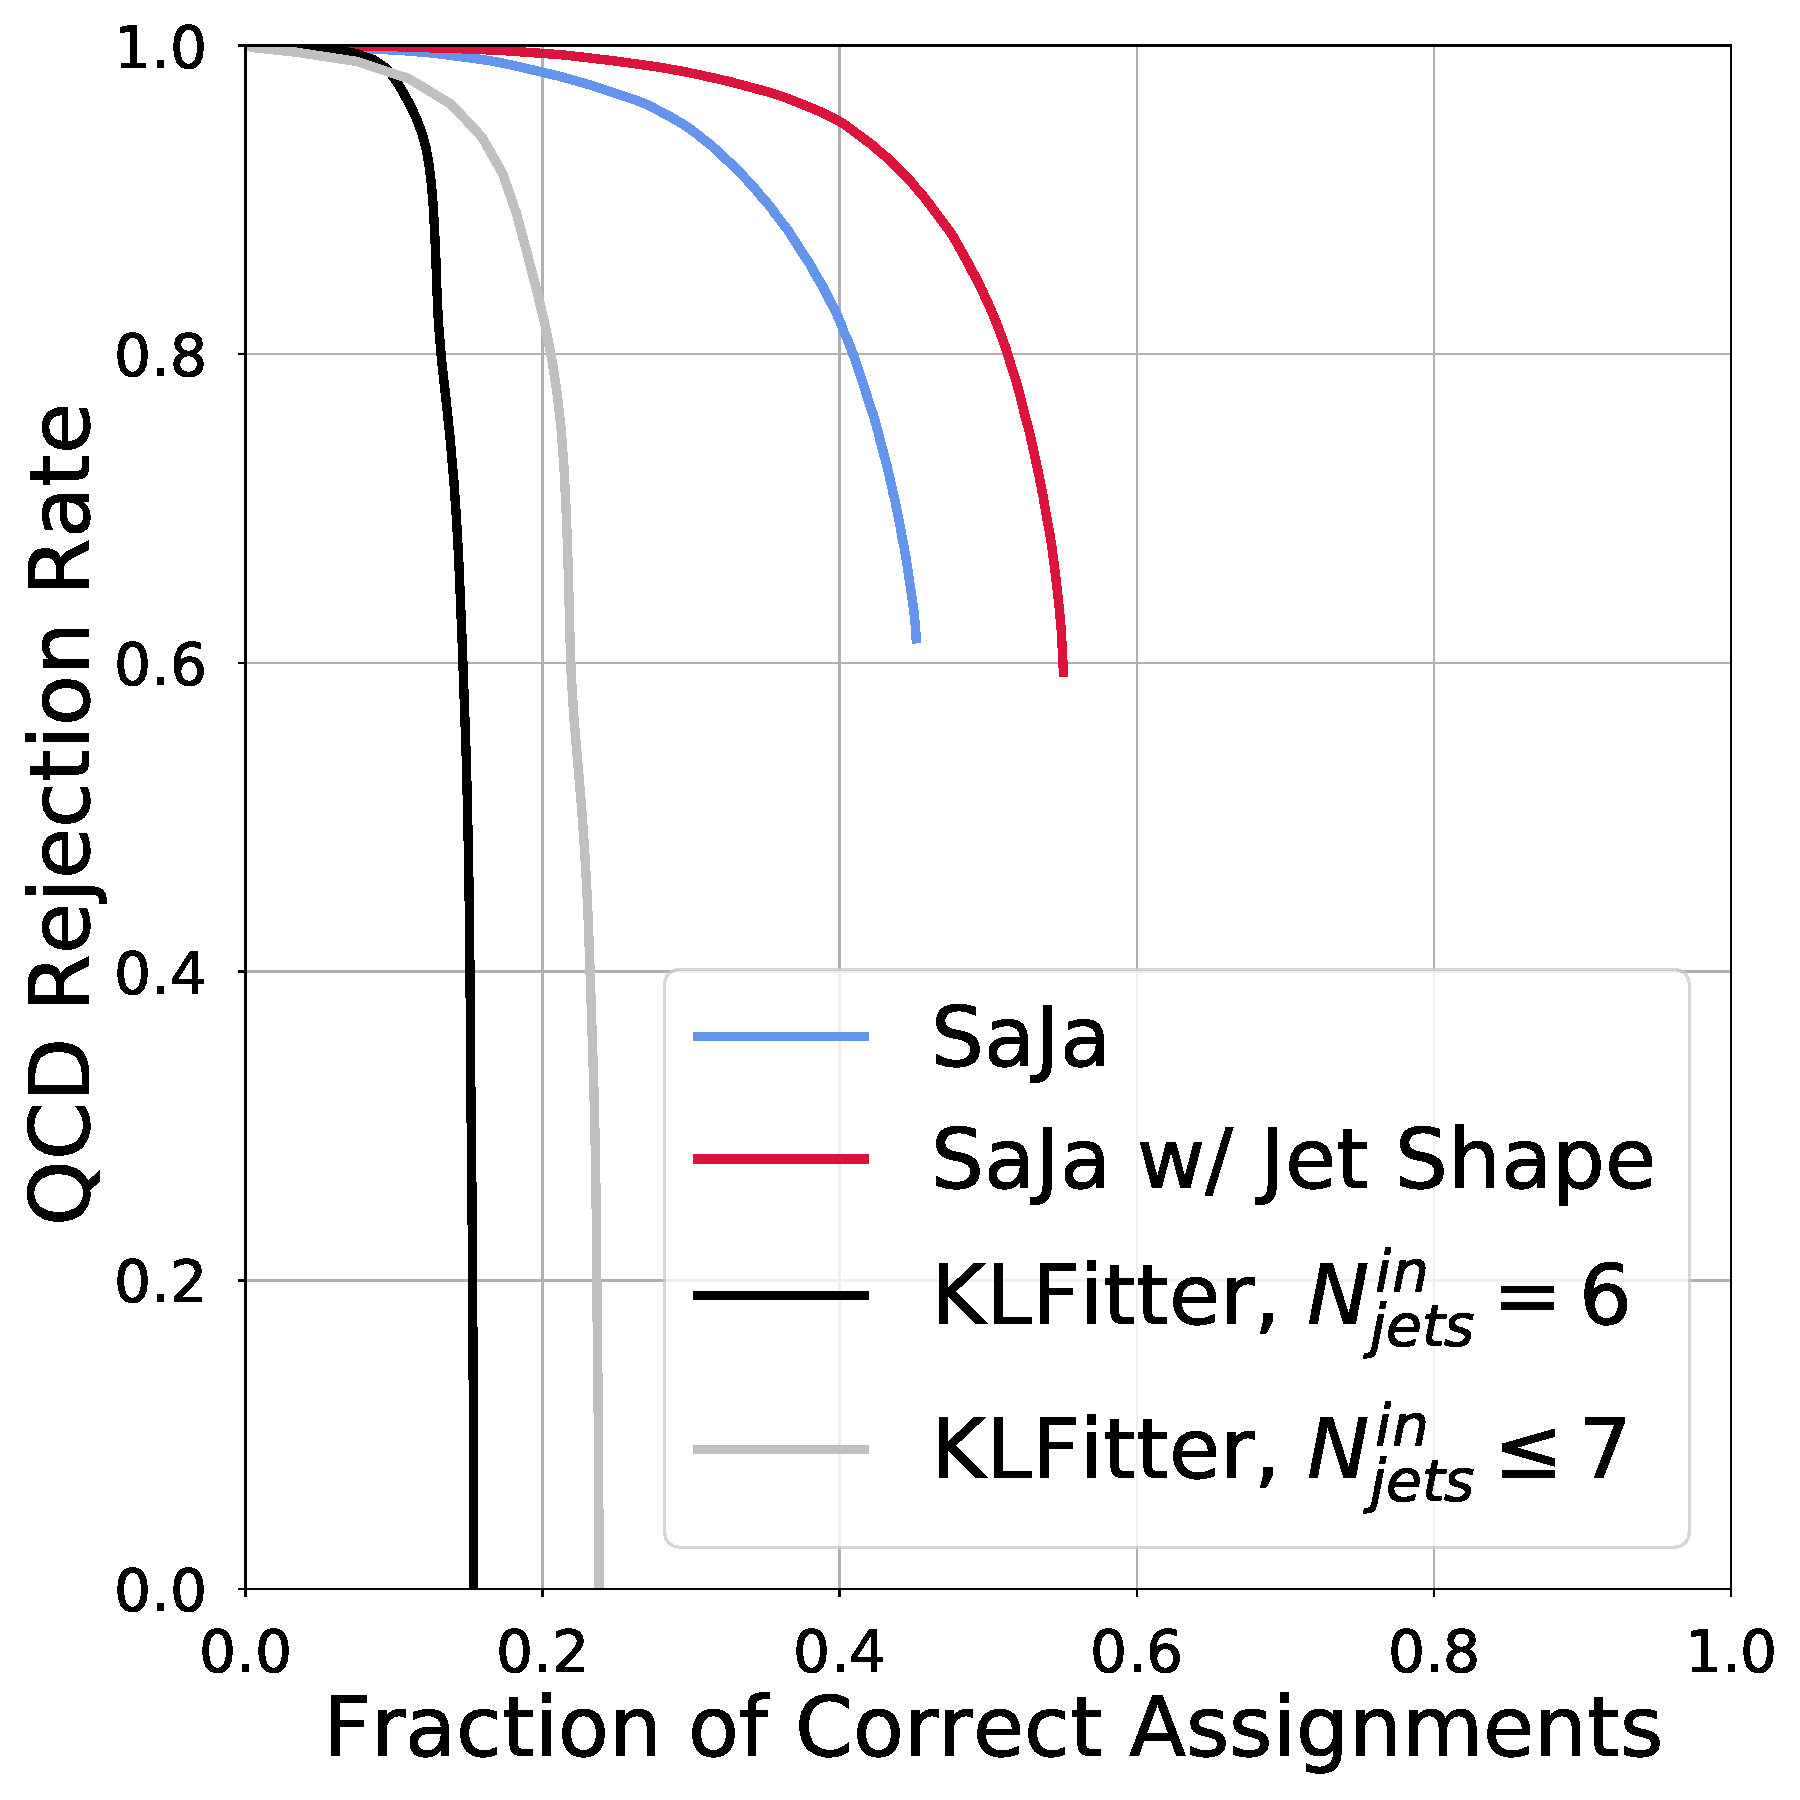
\includegraphics[height=0.32\textheight]{fig/roc/roc_qcd_rej_vs_correct.pdf}
      \end{figure}
  \end{columns}
\end{frame}

%%%%%%%%%%%%%%%%%%%%%%%%%%%%%%%%%%%%%%%%%%%%%%%%%%%%%%%%%%%%%%%%%%%%%%%%%%%%%%%
\begin{frame}[fragile]{Model Interpretability}
  \begin{figure}
    \centering
    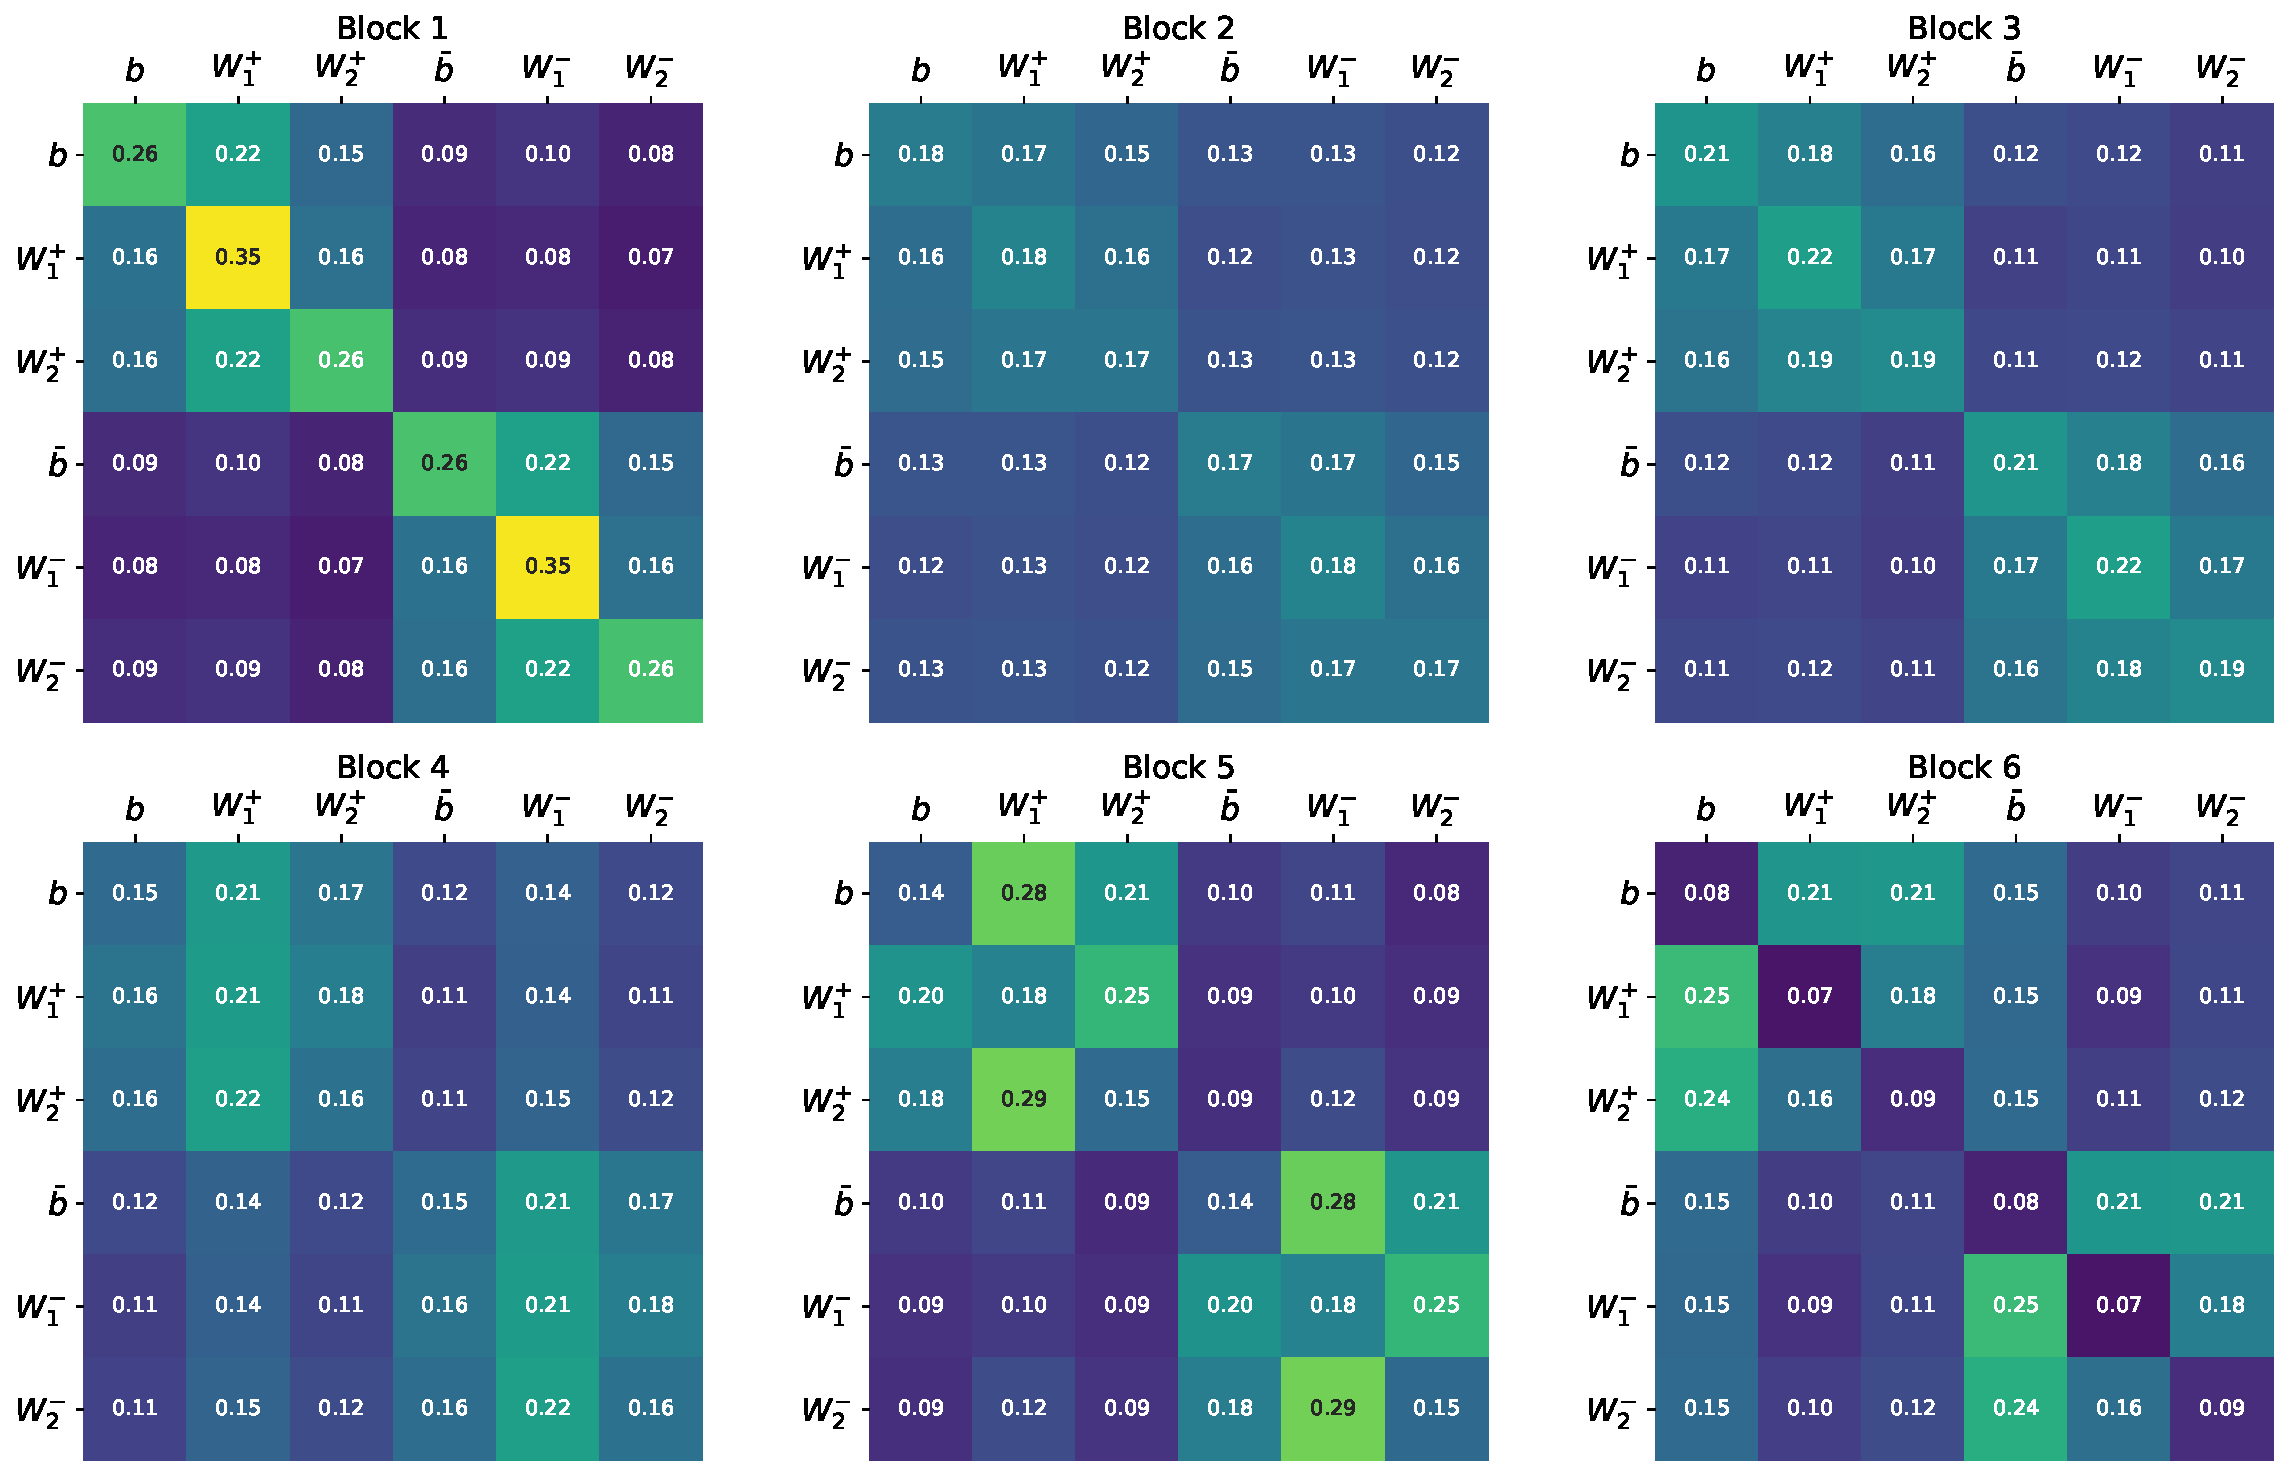
\includegraphics[width=0.75\textwidth]{fig/attention-matrix/attention_tt_mg5_pythia8_alljets_dR-0.30_test_delphys_minmax_jet-shape_correct.pdf}
  \end{figure}
  
  {\footnotesize
    \begin{itemize}
      \item The average of attention matrices for the correct assignments in the matched \ttbar events.
      \item Since \saja, is invariant under the permutation of the jets,
            it is possible to sort the jets using the jet-parton matching information w.l.o.g., for display purposes.
      \item $W_{1}^{+}$ indicates higher \pt one of the two quarks, the decay products of $W^{+}$ boson.
    \end{itemize}
  }
\end{frame}

%%%%%%%%%%%%%%%%%%%%%%%%%%%%%%%%%%%%%%%%%%%%%%%%%%%%%%%%%%%%%%%%%%%%%%%%%%%%%%%
\begin{frame}[fragile]{Summary}
  \begin{itemize}
    \item[$\bullet$] \textsc{SaJa}\, network for jet-parton assignment without jet permutations.
    \item[$\bullet$] \textsc{SaJa}\, shows better jet-parton assignment and background rejection performance compared to \textsc{KLFitter}.
    \item[$\bullet$] Predictive entropy makes it possible to improve performance without additional training.
  \end{itemize}
\end{frame}
